% !TeX program = xelatex
\documentclass{ctexart}
\usepackage{template_by_mny}
\usepackage{float} 

\title{傅里叶光学实验报告}
\class{物理 32/物理 31}
\name{冯家琦/周方远}
\id{2023011338/2023011263}

\begin{document}
\maketitle

\begin{abstract}
  本实验旨在通过搭建傅里叶光学系统,观察并理解光波的衍射、成像、滤波等基本现象,
  并探究傅里叶光学在光学成像中的应用。
\end{abstract}

\section{实验原理}
傅里叶光学是研究光波经过光学系统后的衍射和成像规律的科学。
。在光学显微镜中,物体经过物镜衍射后,其衍射图样会分布在物镜的像平面(即傅里叶平面)上。傅里叶平面上的信息包含了物体的全部信息,通过控制傅里叶平面上的滤波器,可以实现对物体成像的调节。
本实验采用4f光学系统,利用透镜对光波进行变换,在傅里叶平面上观察到光波的频谱信息,并通过滤波等手段实现对图像的处理。

\section{实验仪器}
  仪器:傅里叶光学教学套件 (EDU-FOP2):LED光源、准直透镜、物镜、
  套筒透镜、相机、Targetlens、Condenser lens、Aperture Iris、
  Field Iris、Projection lens、观察屏、分束器、滤光片、Mask

\section{实验步骤}
我们注意到,中文实验说明书上大概以第7个实验为界限,前后光路搭建的顺序并不相同,因此我们在第七个实验后
将实验仪器拆卸后重新以另一个顺序搭建。

1. 搭建4f光学系统,按照文档中提供的步骤进行调节,确保各个光学元件的高度、位置和角度正确。

2. 使用相机观察Target上的图案,并通过调节焦距和曝光时间获得清晰的图像。

3. 调节分束器和Projection lens,将傅里叶平面上的图像投射到观察屏上。

4. 进行以下实验内容:

\subsection{开普勒望远镜成像}
将Field lens和Condenser lens依次摆在光源前,并使两者间隔为两者焦距之和。将Target放在光源与Field lens之间,将屏放置在Condenser lens后焦平面处,观察到倒立缩小的图像。

\begin{figure}[htbp]
  \centering
  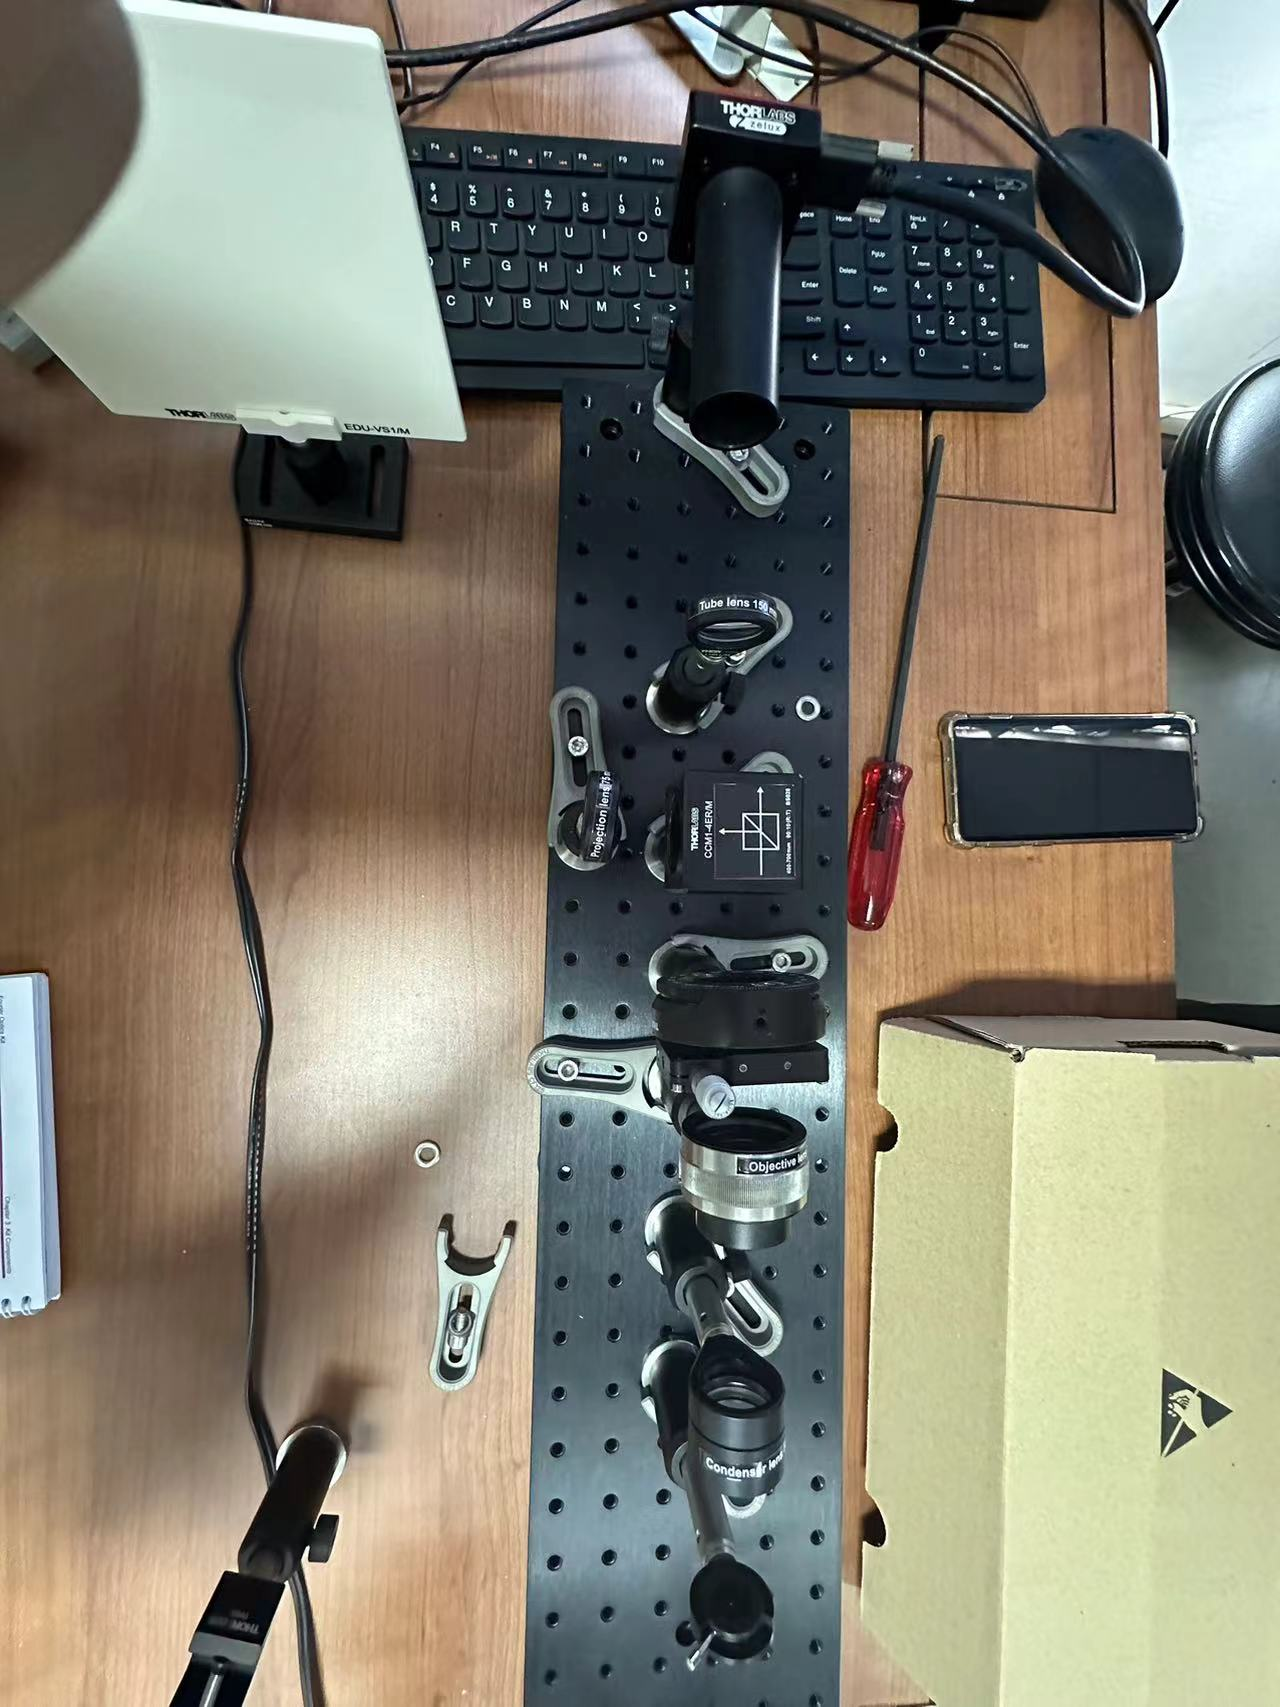
\includegraphics[width=0.2\textwidth,height=0.3\textwidth]{pictures/微信图片_20241010200924.jpg}
  \caption{开普勒望远镜仪器安装}
\end{figure} 

\subsection{开普勒望远镜(Condenser lens+ Objective lens)}
• 将物镜(f = 30 mm) 放在 Condenser lens (f = 50 mm) 后面,使其焦平面重
合;

• 将 Target 放在 Condenser lens 的 LED 侧焦平面上,然后将观察屏放在 O 物镜的后
焦平面上观察图像,观察到倒立缩小的图像。
\begin{figure}[htbp]
  \centering
  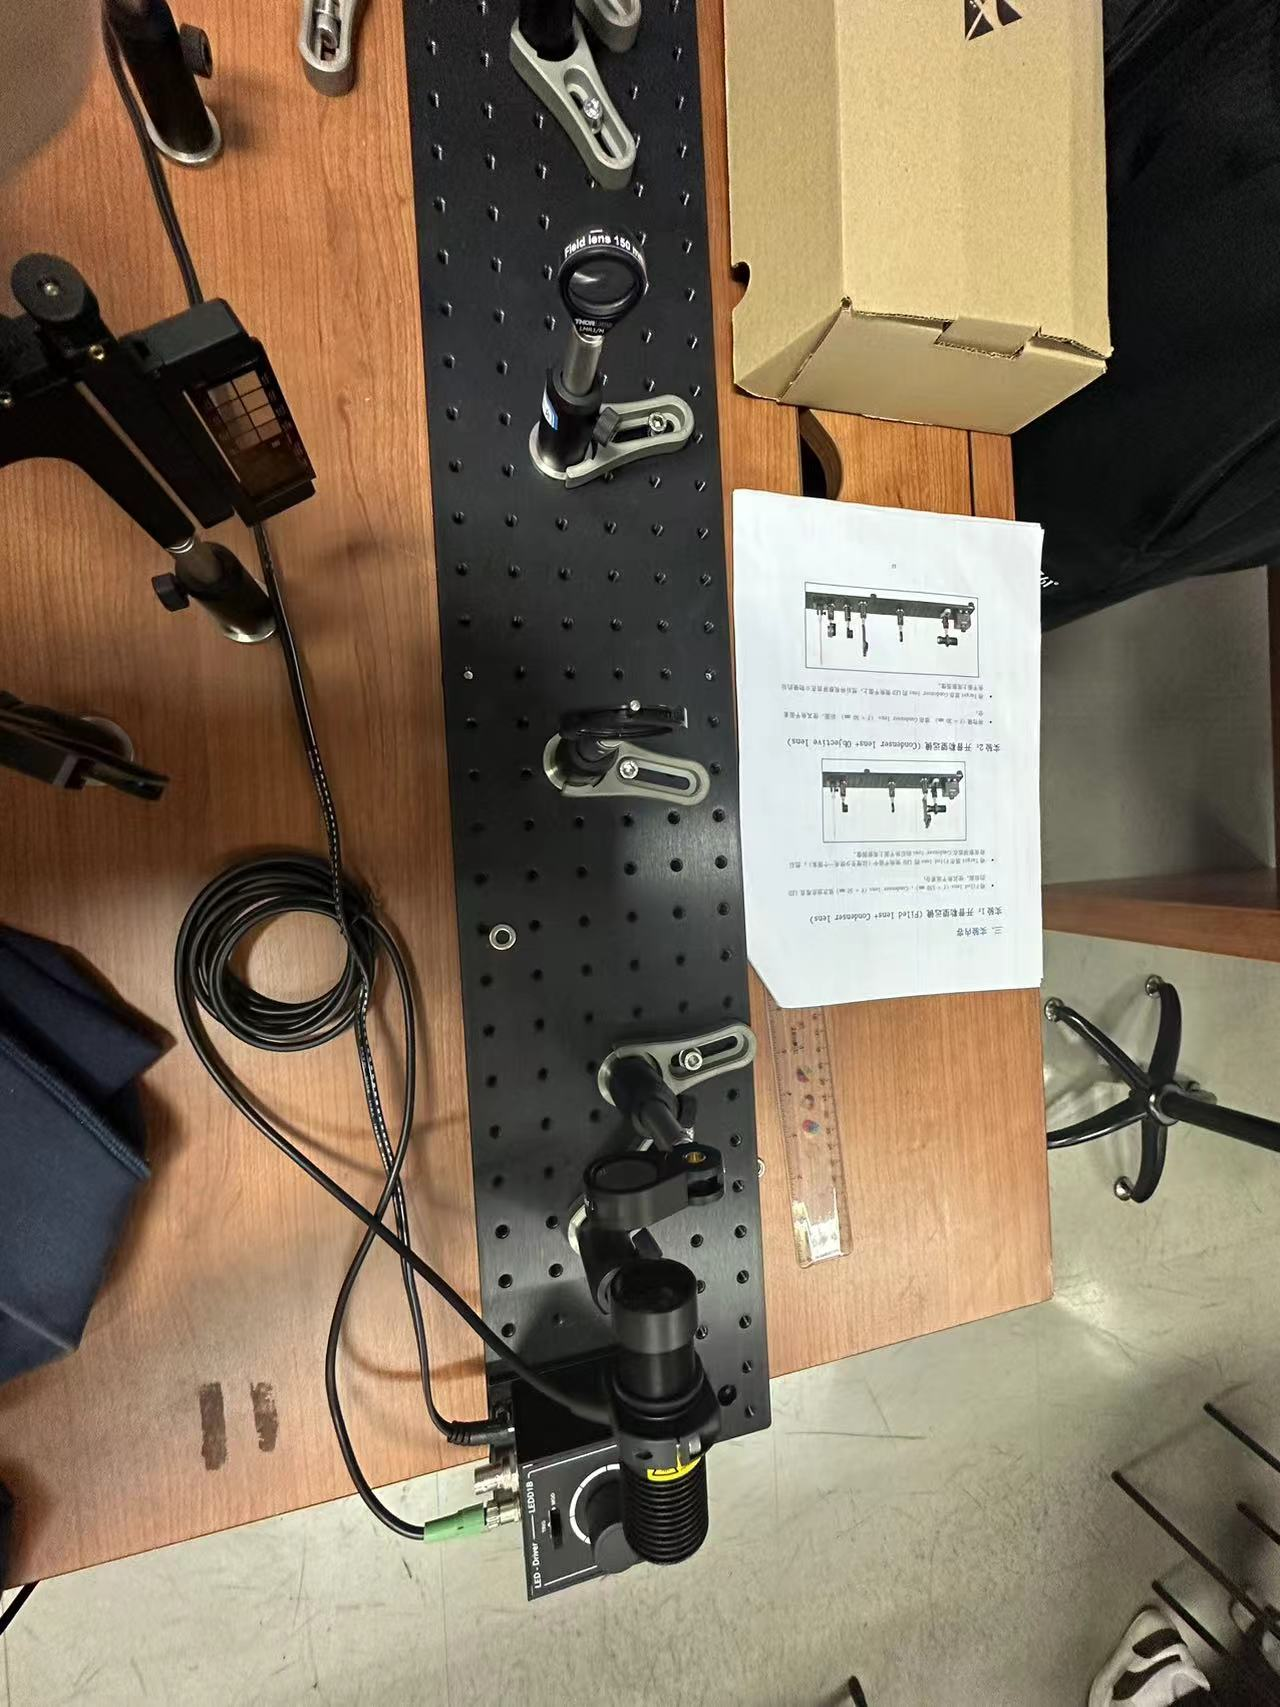
\includegraphics[width=0.2\textwidth,height=0.3\textwidth]{pictures/微信图片_20241010200942.jpg}
  \caption{开普勒望远镜仪器安装}
\end{figure} 
\subsection{Projection lens成像}
\begin{figure}[htbp]
  \centering
  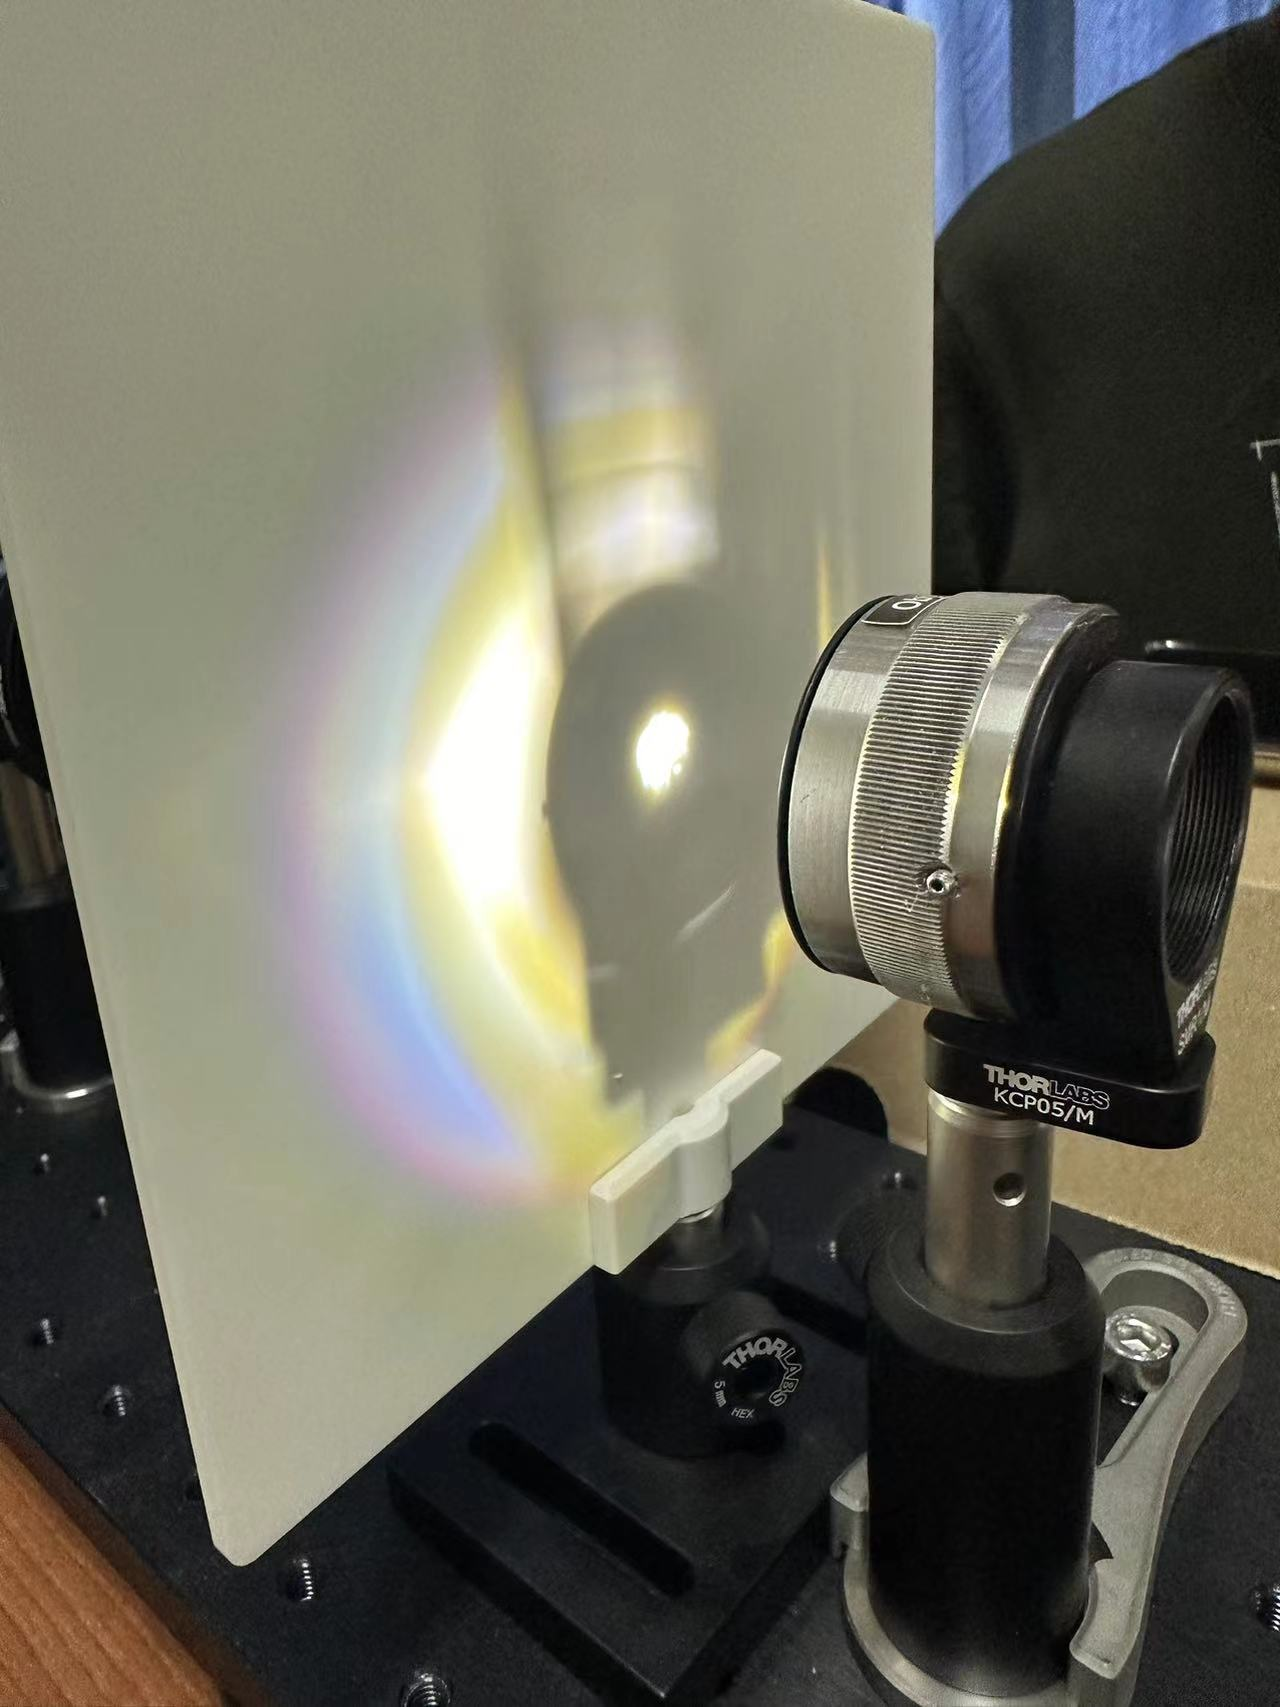
\includegraphics[width=0.2\textwidth,height=0.3\textwidth]{pictures/微信图片_20241010200955.jpg}
  \caption{Projection lens成像}
\end{figure} 
\subsection{观察傅里叶面}
• 调整 Target 找到晶格(例如:第一行 F2 图案,g = 15 μm,b = 6 μm 晶格)图
案的位置,在相机上看到晶格图像的同时可以在观察屏上看到该晶格图案的清晰的
傅里叶图像
\begin{figure}[htbp]
  \centering
  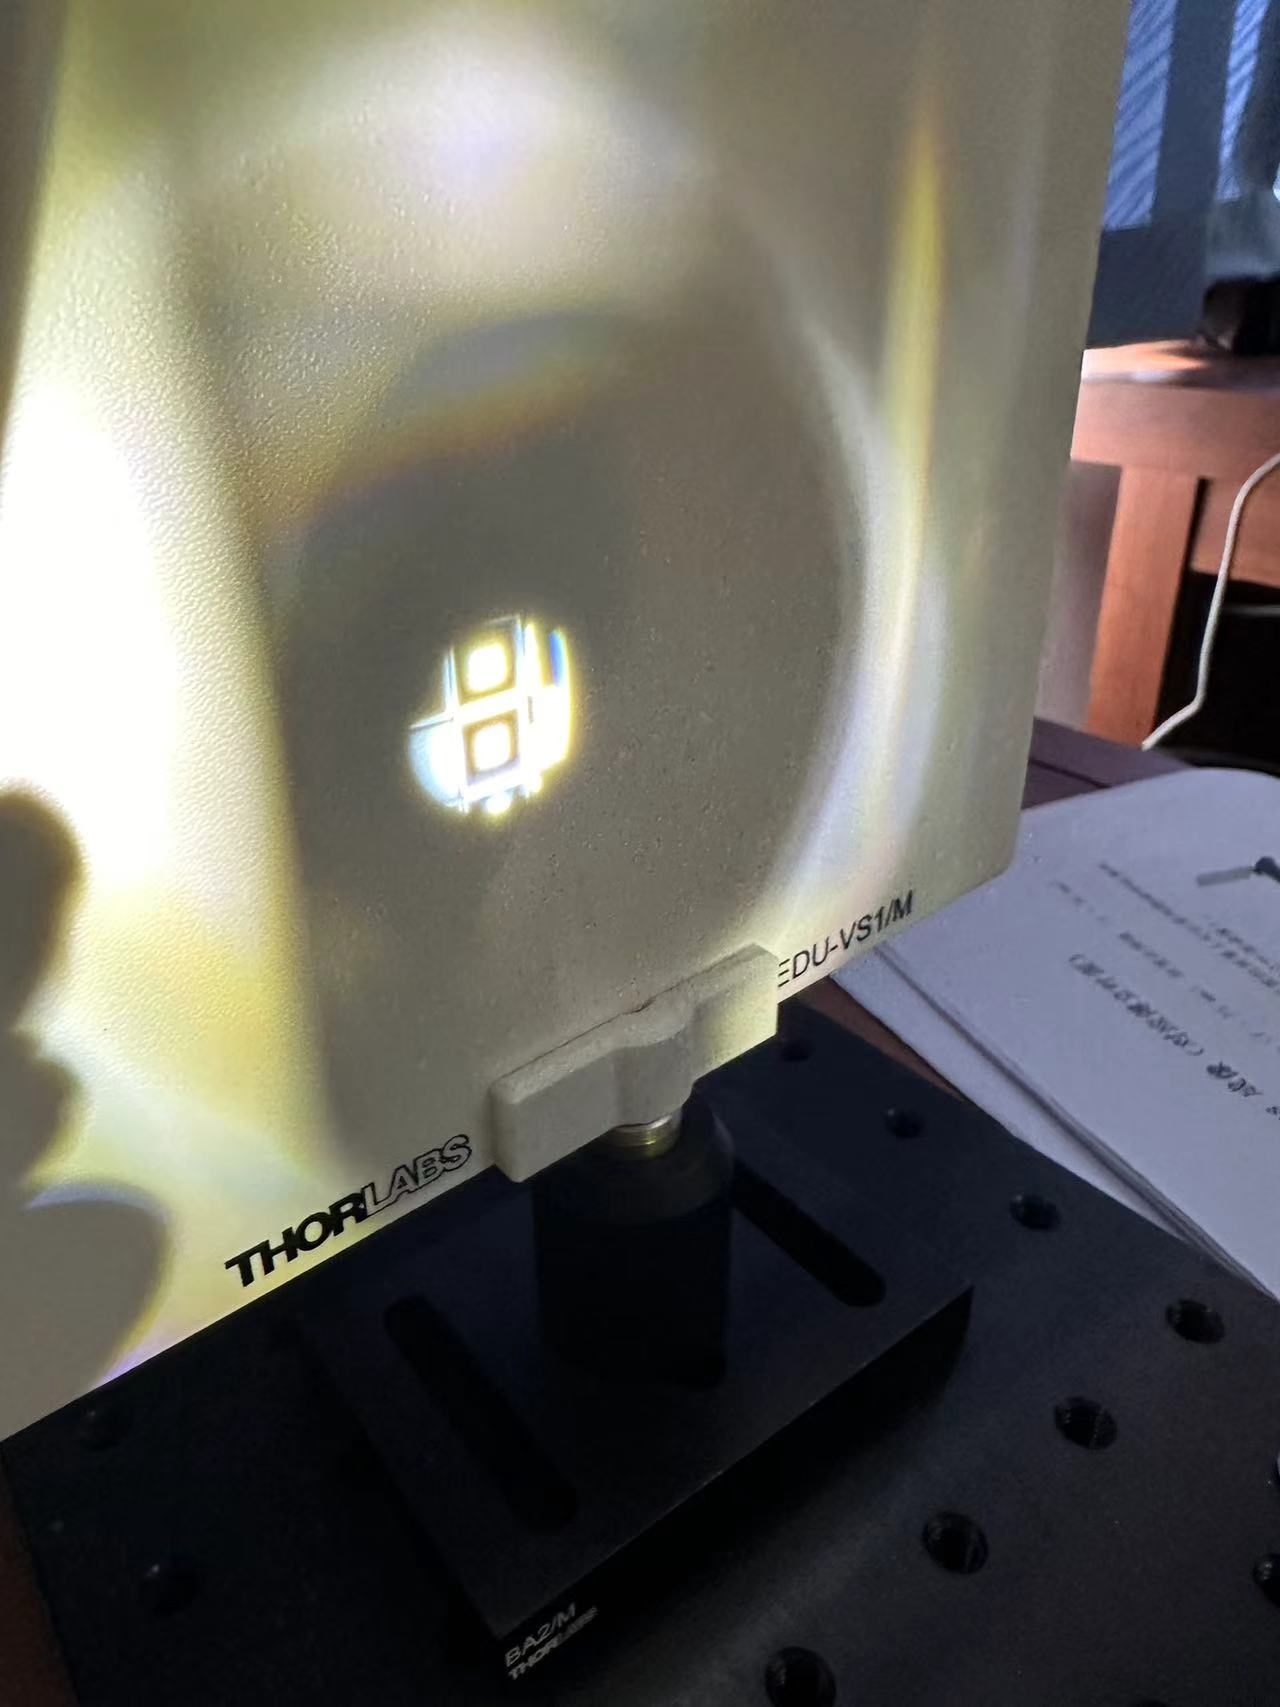
\includegraphics[width=0.2\textwidth,height=0.3\textwidth]{pictures/微信图片_20241010201008.jpg}
  \caption{观察傅里叶面} 
\end{figure}
\subsection{Field Iris和Aperture Iris的作用}
• Field Iris控制物体照明区域,影响图像亮度。

• Aperture Iris控制成像系统孔径,影响图像分辨率和衍射斑形状。
\begin{figure}[H]
  \centering
  \begin{minipage}[b]{0.2\textwidth}
    \centering
    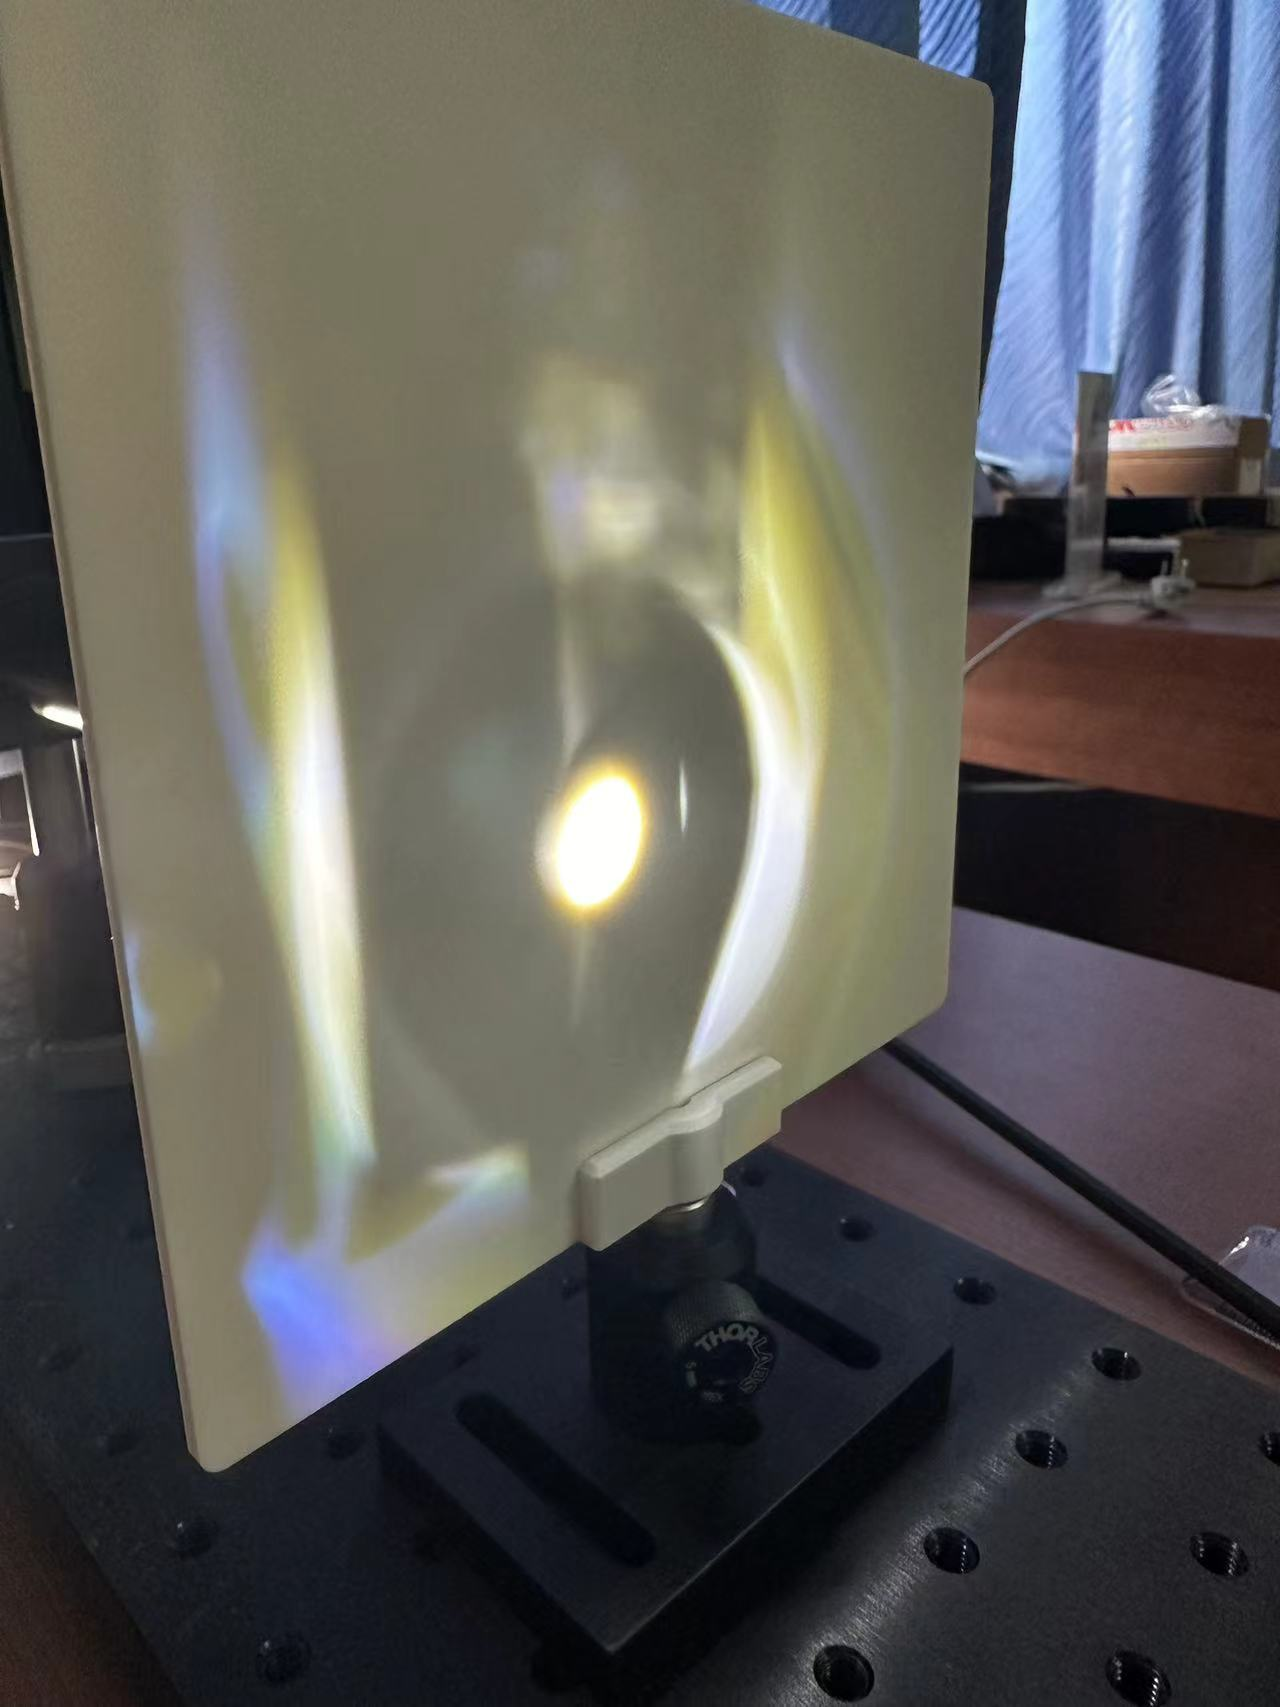
\includegraphics[width=\textwidth]{pictures/微信图片_20241010201015.jpg}
    \caption{Field Iris和Aperture Iris都开}
  \end{minipage}
  \hspace{0.05\textwidth} % 图片之间的水平间距
  \begin{minipage}[b]{0.2\textwidth}
    \centering
    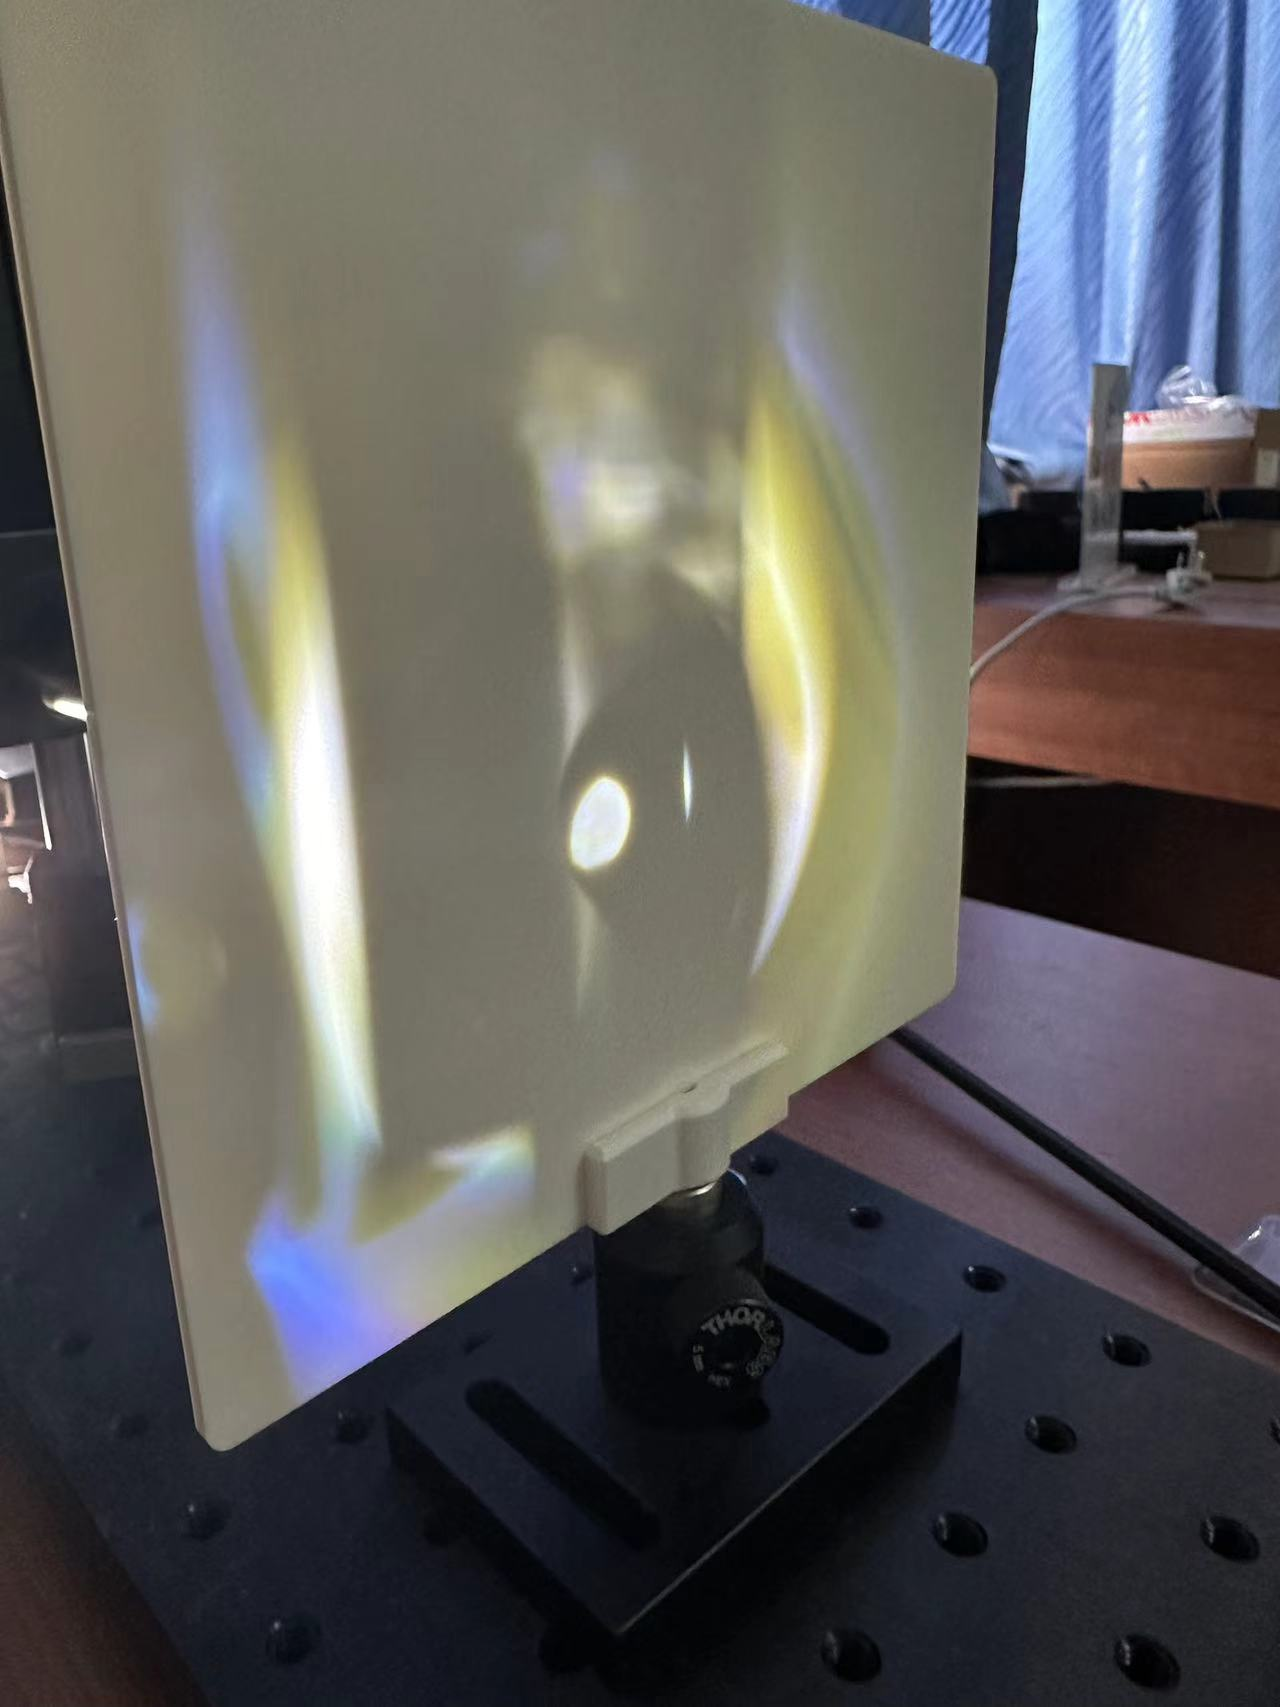
\includegraphics[width=\textwidth]{pictures/微信图片_20241010201018.jpg}
    \caption{Field Iris关,Aperture Iris开}
  \end{minipage}
  \hspace{0.05\textwidth} % 图片之间的水平间距
  \begin{minipage}[b]{0.2\textwidth}
    \centering
    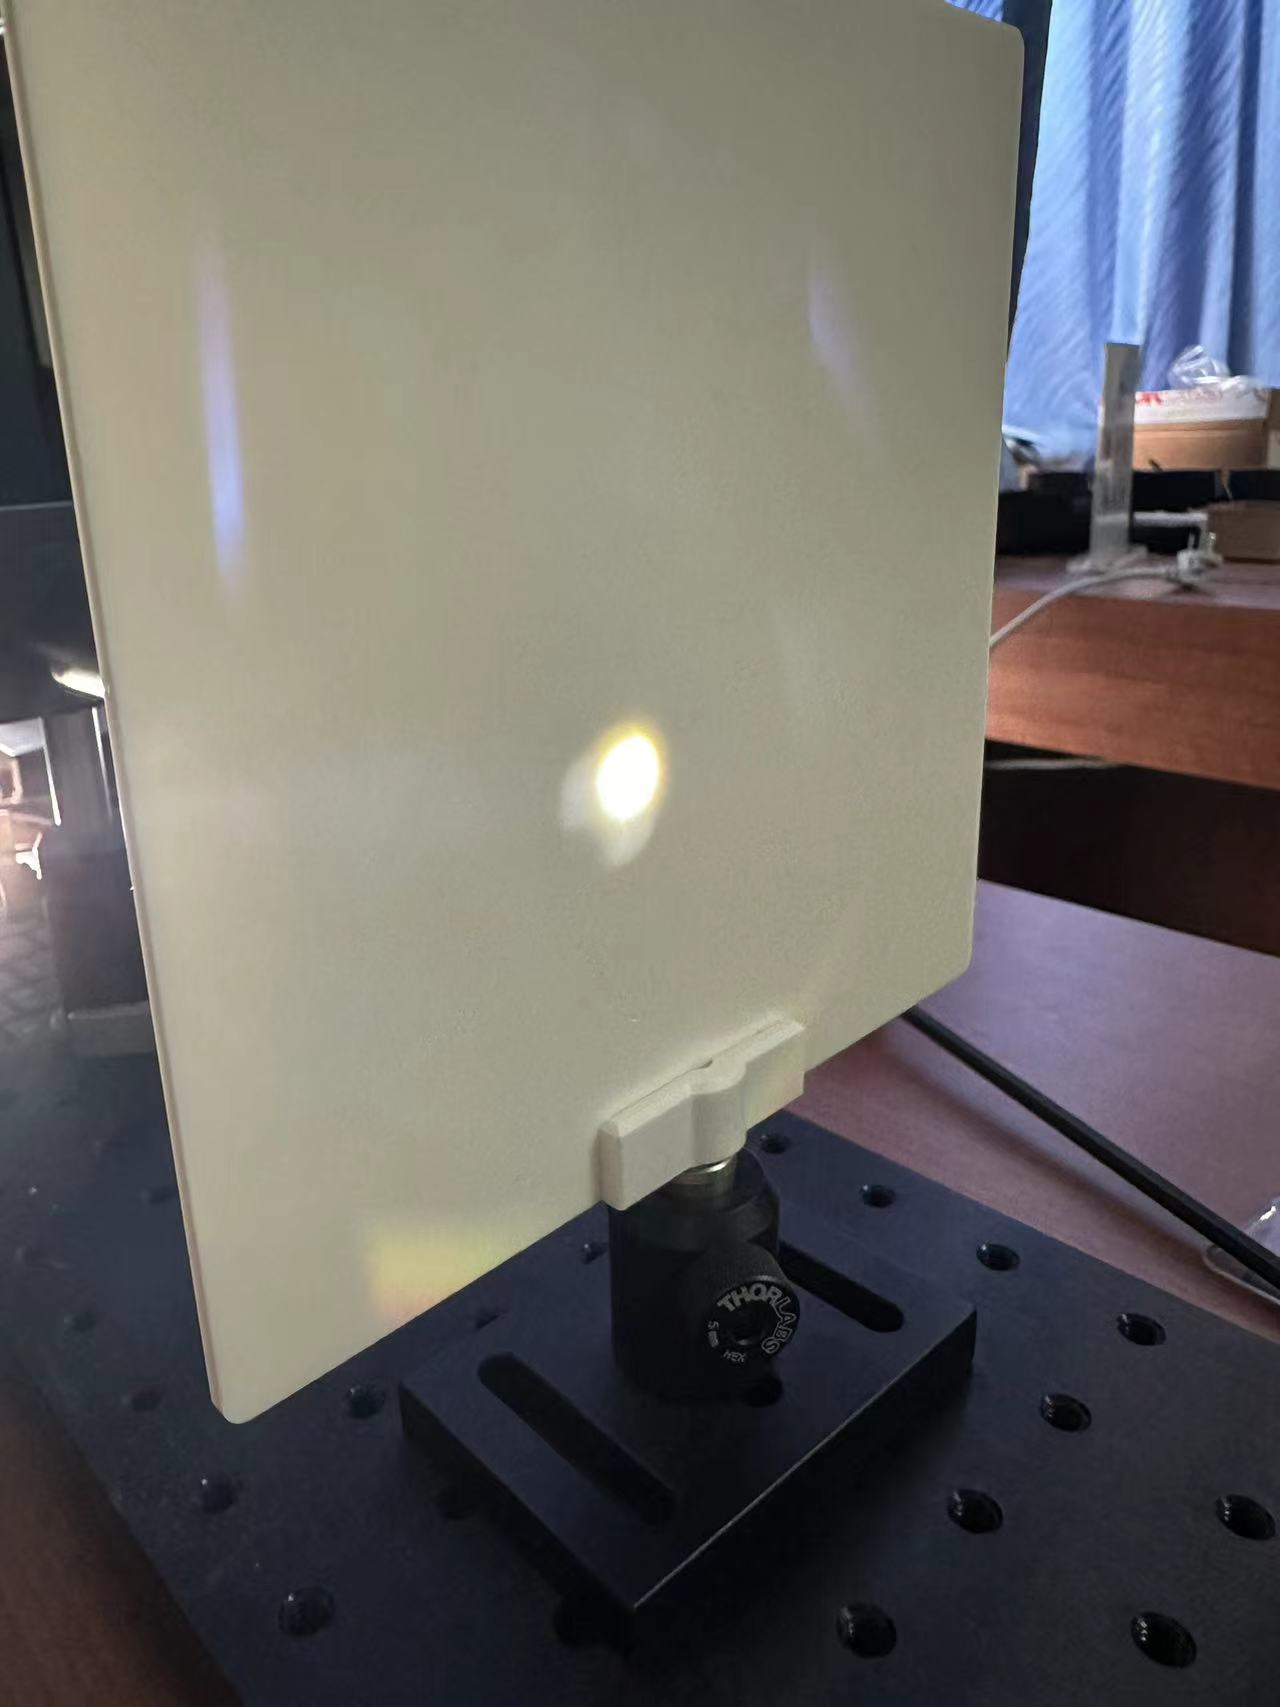
\includegraphics[width=\textwidth]{pictures/微信图片_20241010201022.jpg}
    \caption{Field Iris开,Aperture Iris关}
  \end{minipage}
  \begin{minipage}[b]{0.2\textwidth}
    \centering
    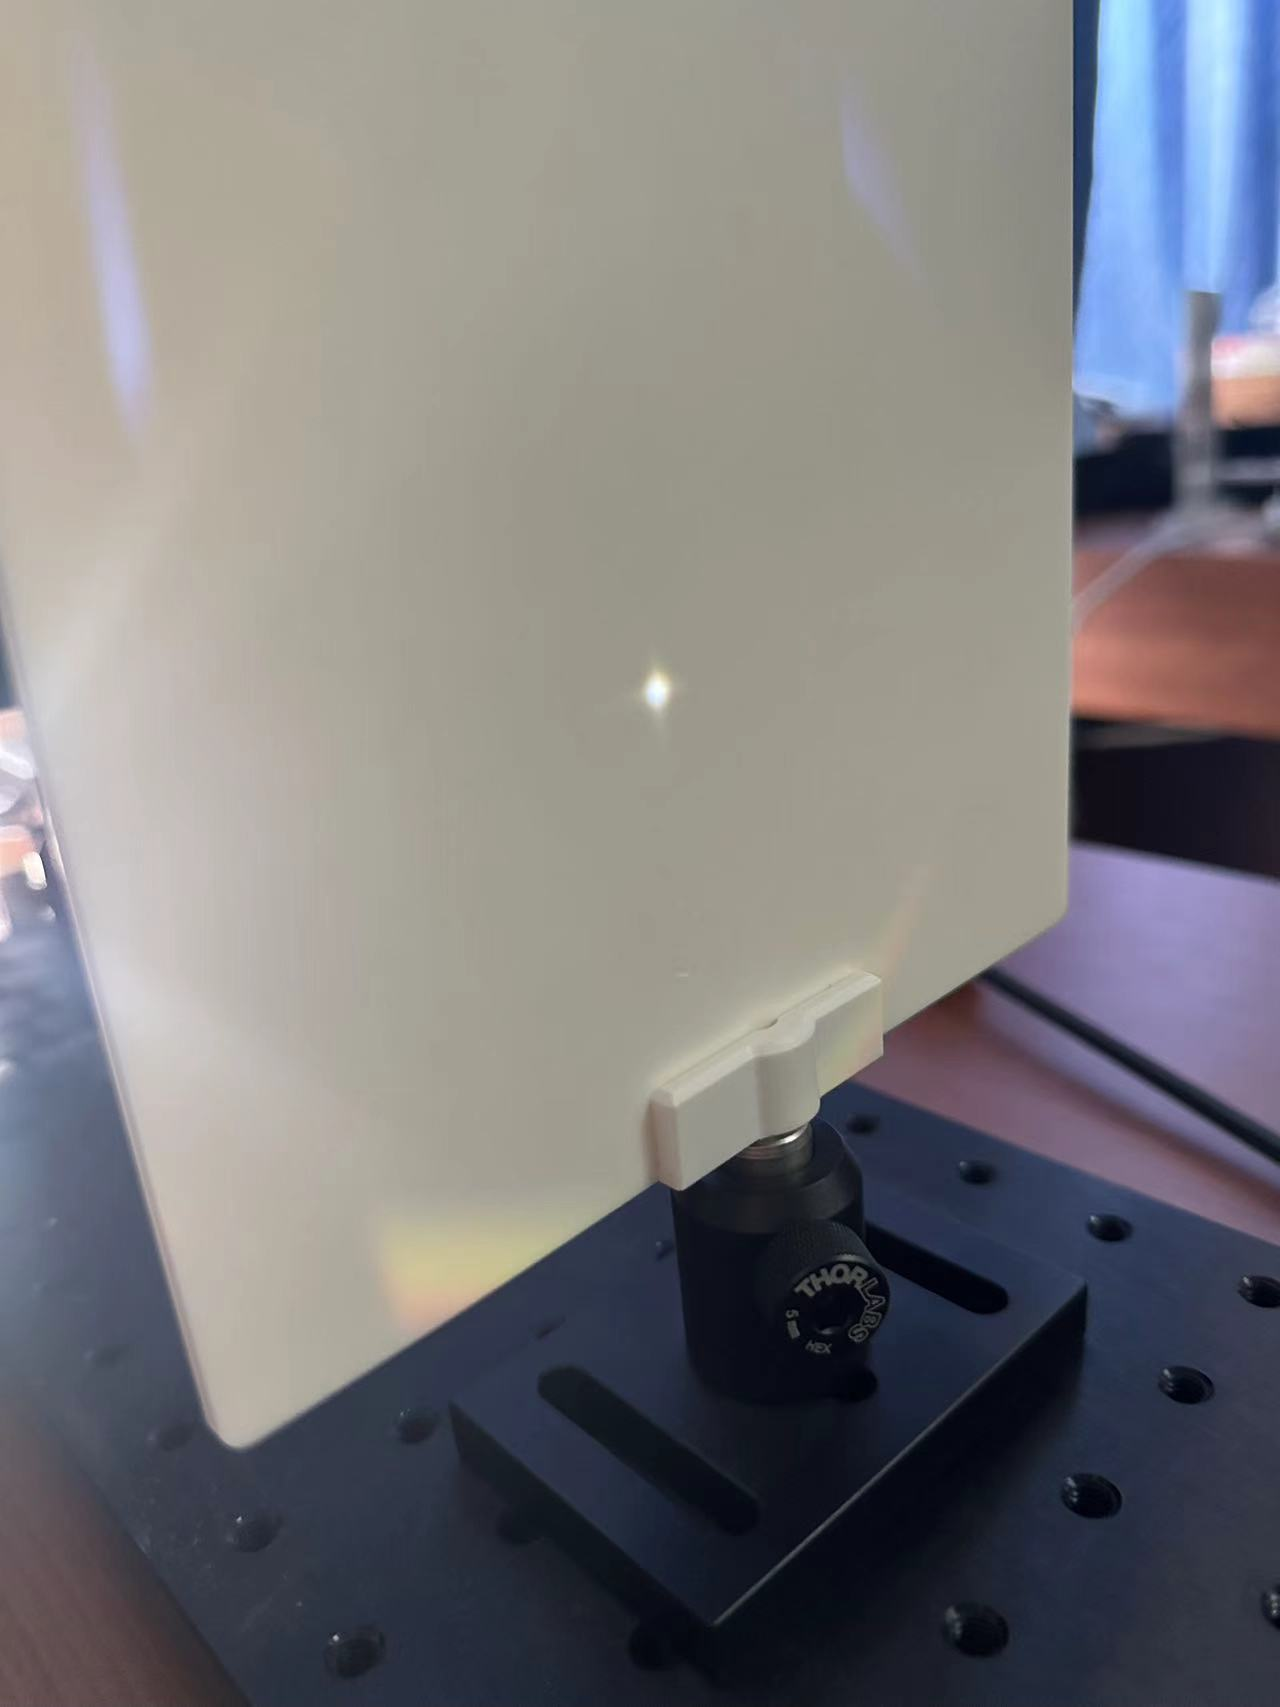
\includegraphics[width=\textwidth]{pictures/微信图片_20241010201025.jpg}
    \caption{Field Iris和Aperture Iris都关}
  \end{minipage}
\end{figure}
\subsection{直接观察 Objective lens 后的傅里叶面}
• 通过直接观察 Objective lens 后的傅里叶面,可以观察到物体的频谱信息。

• 注意要“直接”,不能通过相机观察

• Field Iris和Aperture Iris大概关上1/3较为合适,可以看到清晰的傅里叶面。
\begin{figure}[H]
  \centering
  \begin{minipage}[b]{0.2\textwidth}
    \centering
    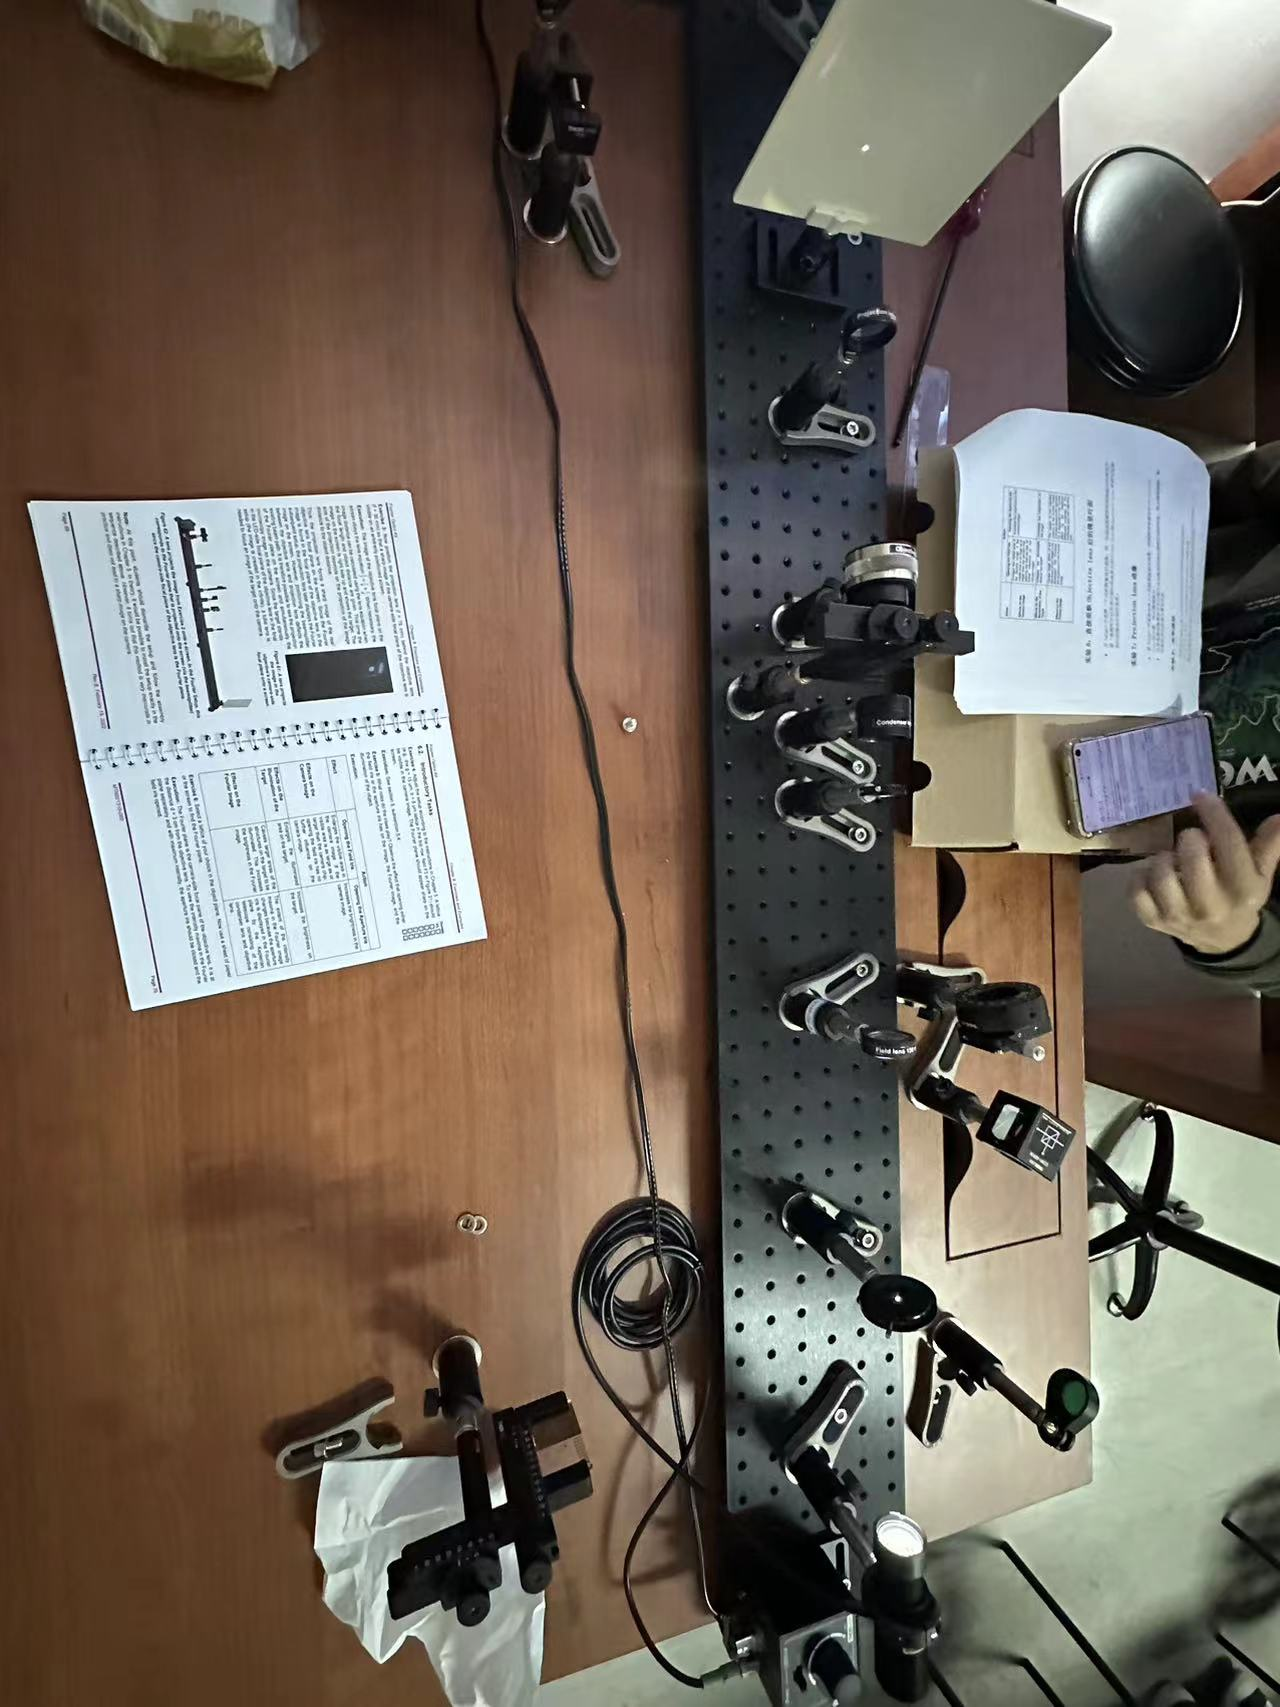
\includegraphics[width=\textwidth]{pictures/微信图片_20241010201028.jpg}
    \caption{仪器摆放}
  \end{minipage}
  \hspace{0.05\textwidth} % 图片之间的水平间距
  \begin{minipage}[b]{0.2\textwidth}
    \centering
    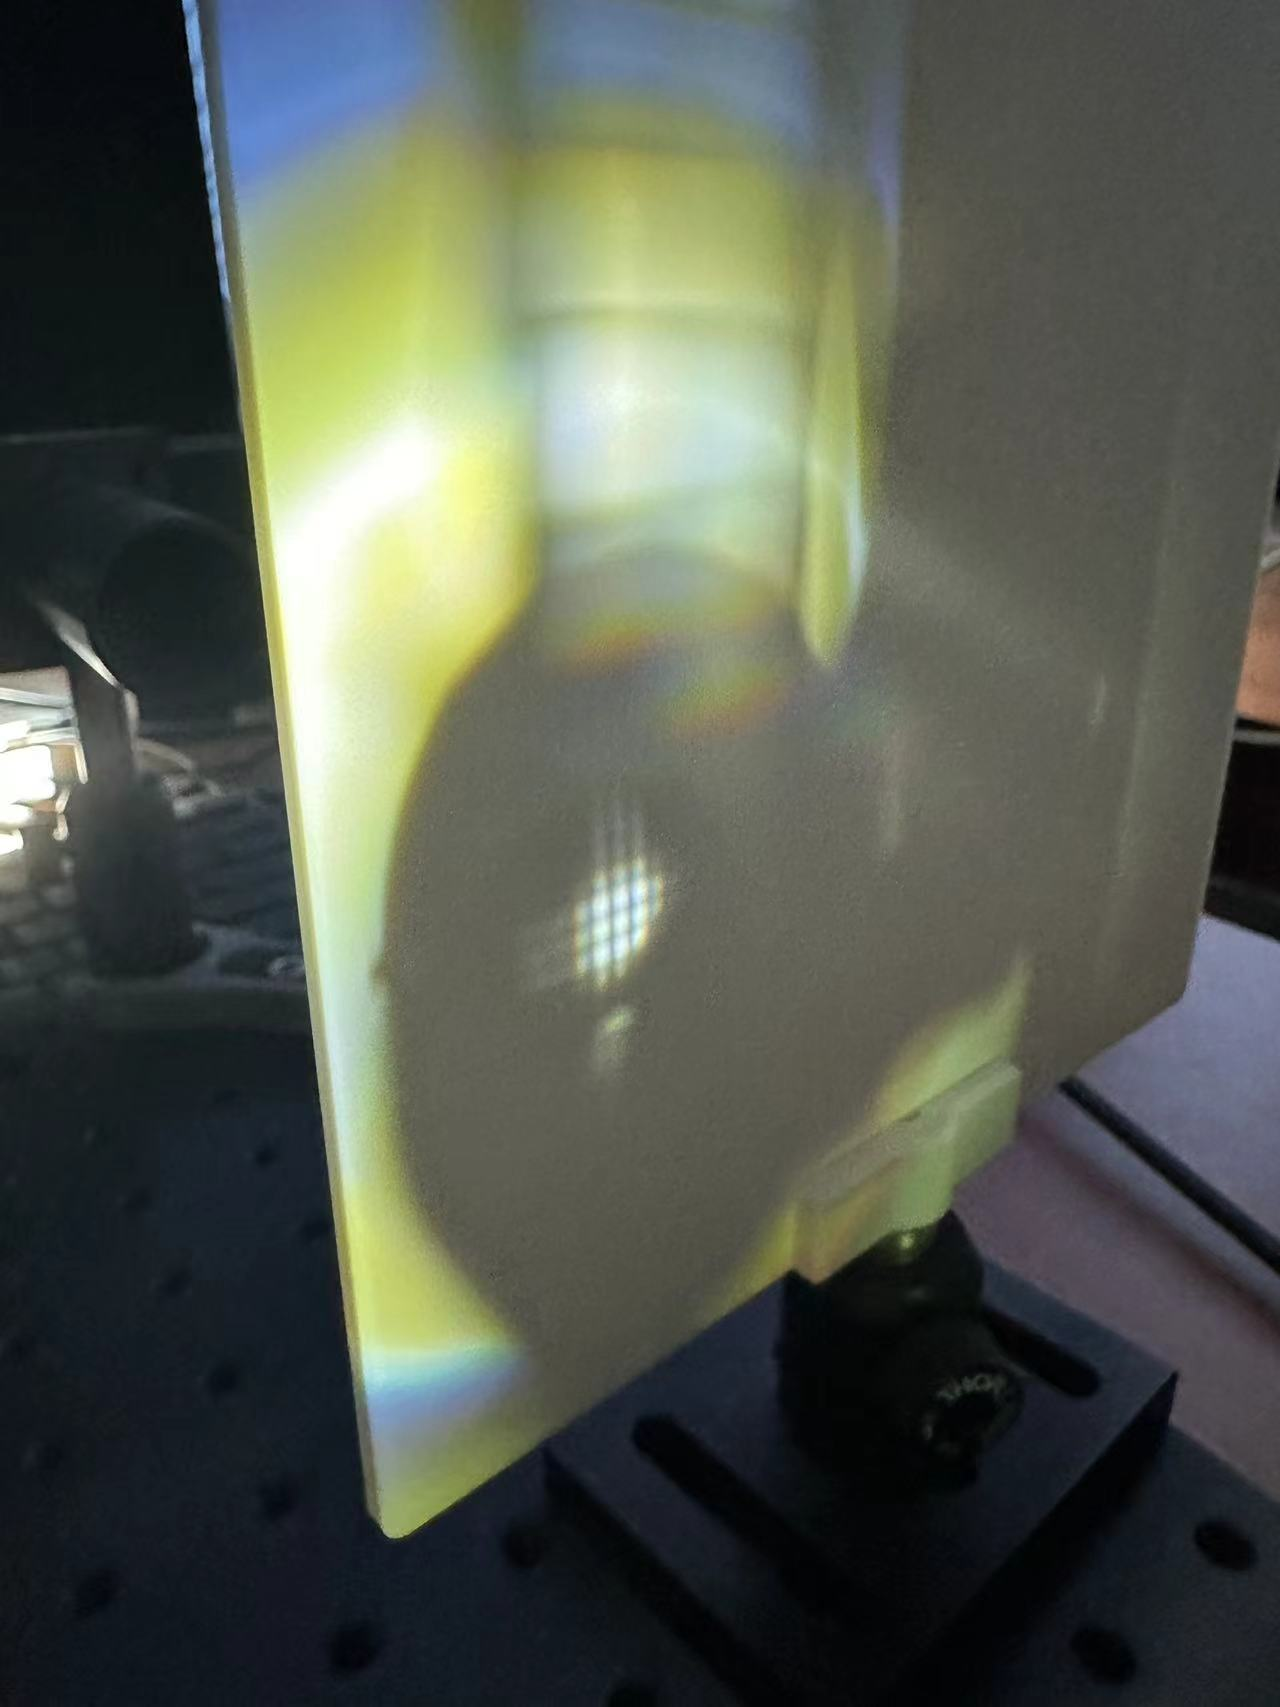
\includegraphics[width=\textwidth]{pictures/微信图片_20241010201031.jpg}
    \caption{点阵图案}
  \end{minipage}
\end{figure}
\subsection{Projection lens 成像}
• 随着屏从前向后移动,图像从清晰到模糊再到显示傅里叶平面的成像,这一变化过程体现了光学成像的原理。
\subsection{光学滤波}
• 先依照文档重新搭建完整的 4f 光学系统。

• 将 Target 放置在物镜光源一侧的焦平面上,将 Mask 放在物镜相机一侧的焦平面上(傅里叶面上)。

• 通过相机观察 Target 上的图像,并利用分束镜和 Projection lens 将傅里叶面投影在远处的观察屏上。
\subsubsection{F2}
调整 Target 上的 F2 图像到光路中,使其能够在相机中清晰成像,并观察屏上的傅里叶图像。
\begin{figure}[H]
  \centering
  \begin{minipage}[b]{0.2\textwidth}
    \centering
    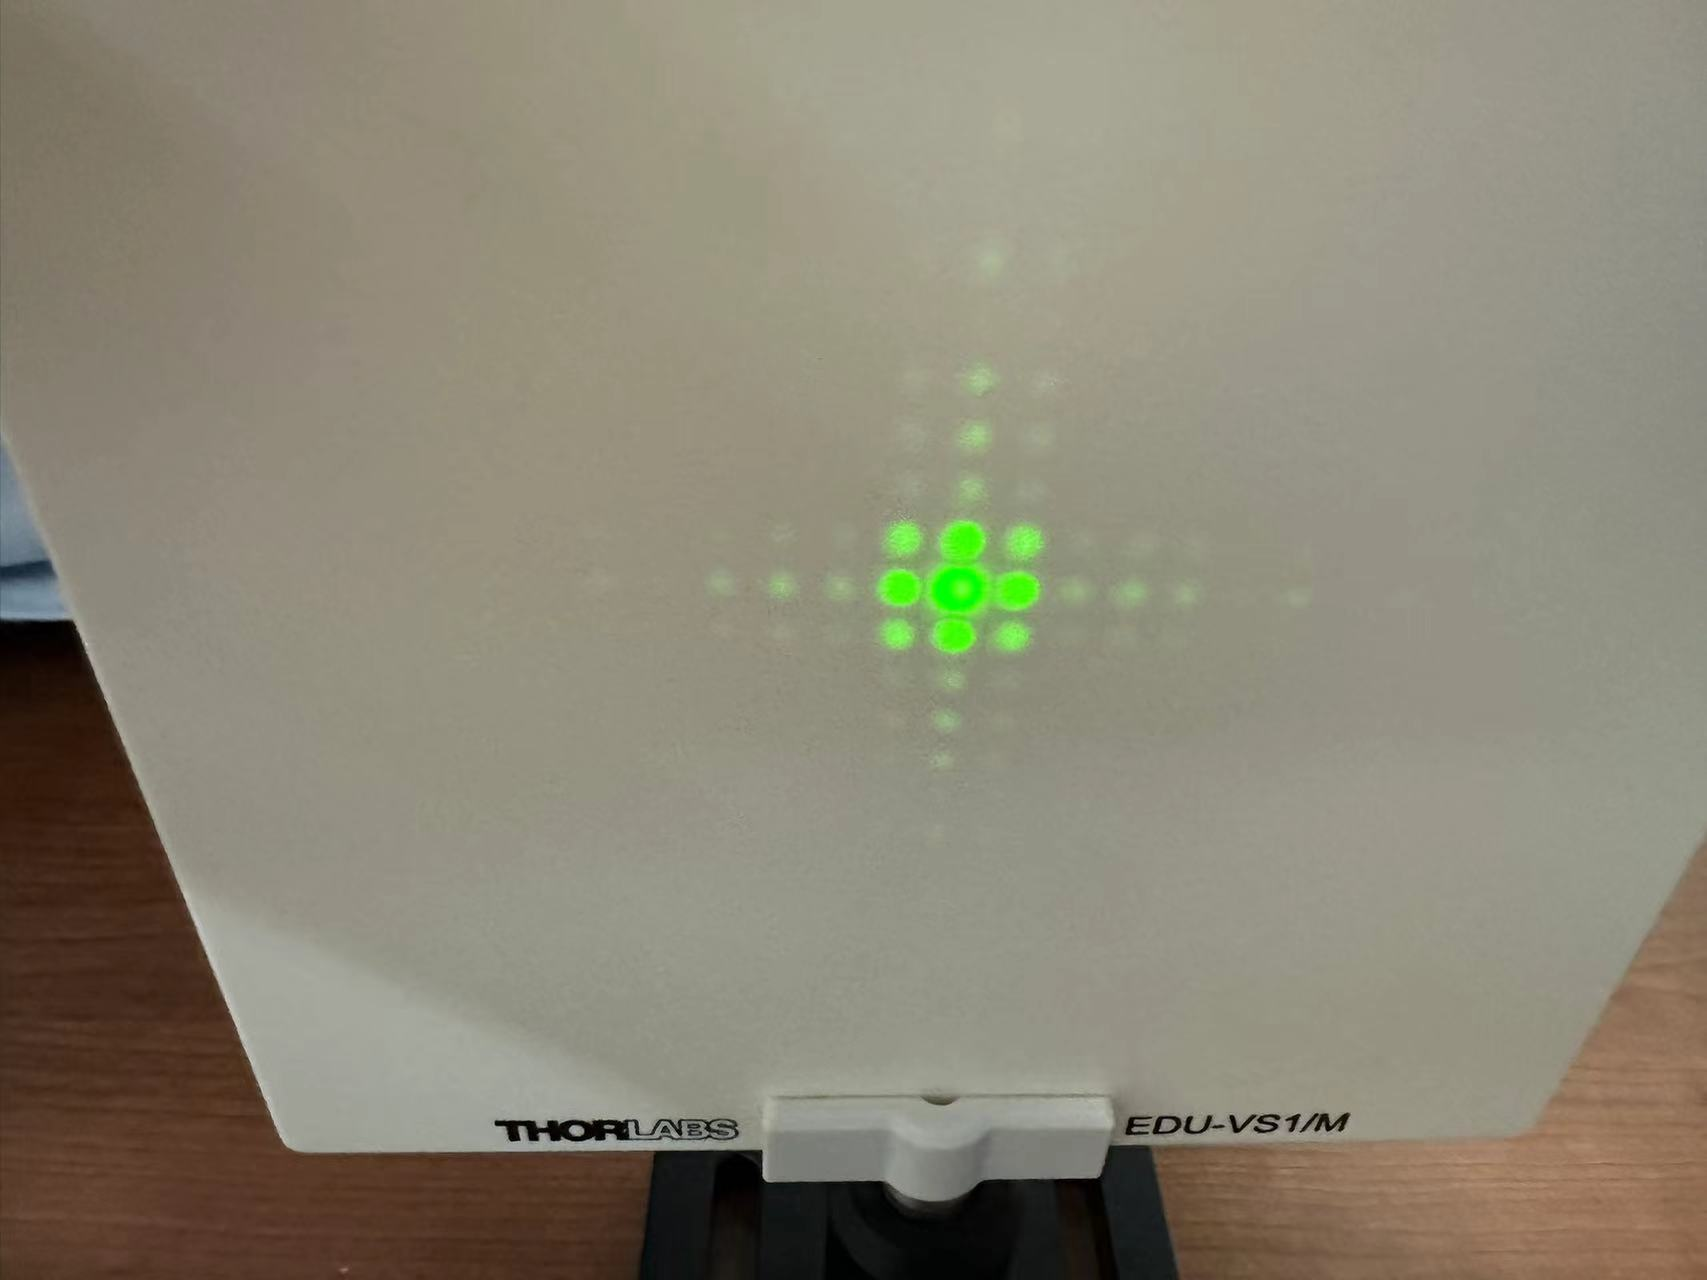
\includegraphics[width=\textwidth]{pictures/微信图片_20241010201054.jpg}
    \caption{F2 傅里叶面}
  \end{minipage}
  \hspace{0.1\textwidth} % 图片之间的水平间距
  \begin{minipage}[b]{0.3\textwidth}
    \centering
    
\includegraphics[width=\textwidth]{pictures/F2-nomask.png}
    \caption{F2 相机成像}
  \end{minipage}
\end{figure}

用 Mask 上的横条纹遮住傅里叶面上除了中间行以外的其他行。观察到相机中的图像变为竖条纹,这是因为仅有水平方向的波数被保留。
\begin{figure}[H]
  \centering
  \begin{minipage}[b]{0.2\textwidth}
    \centering
    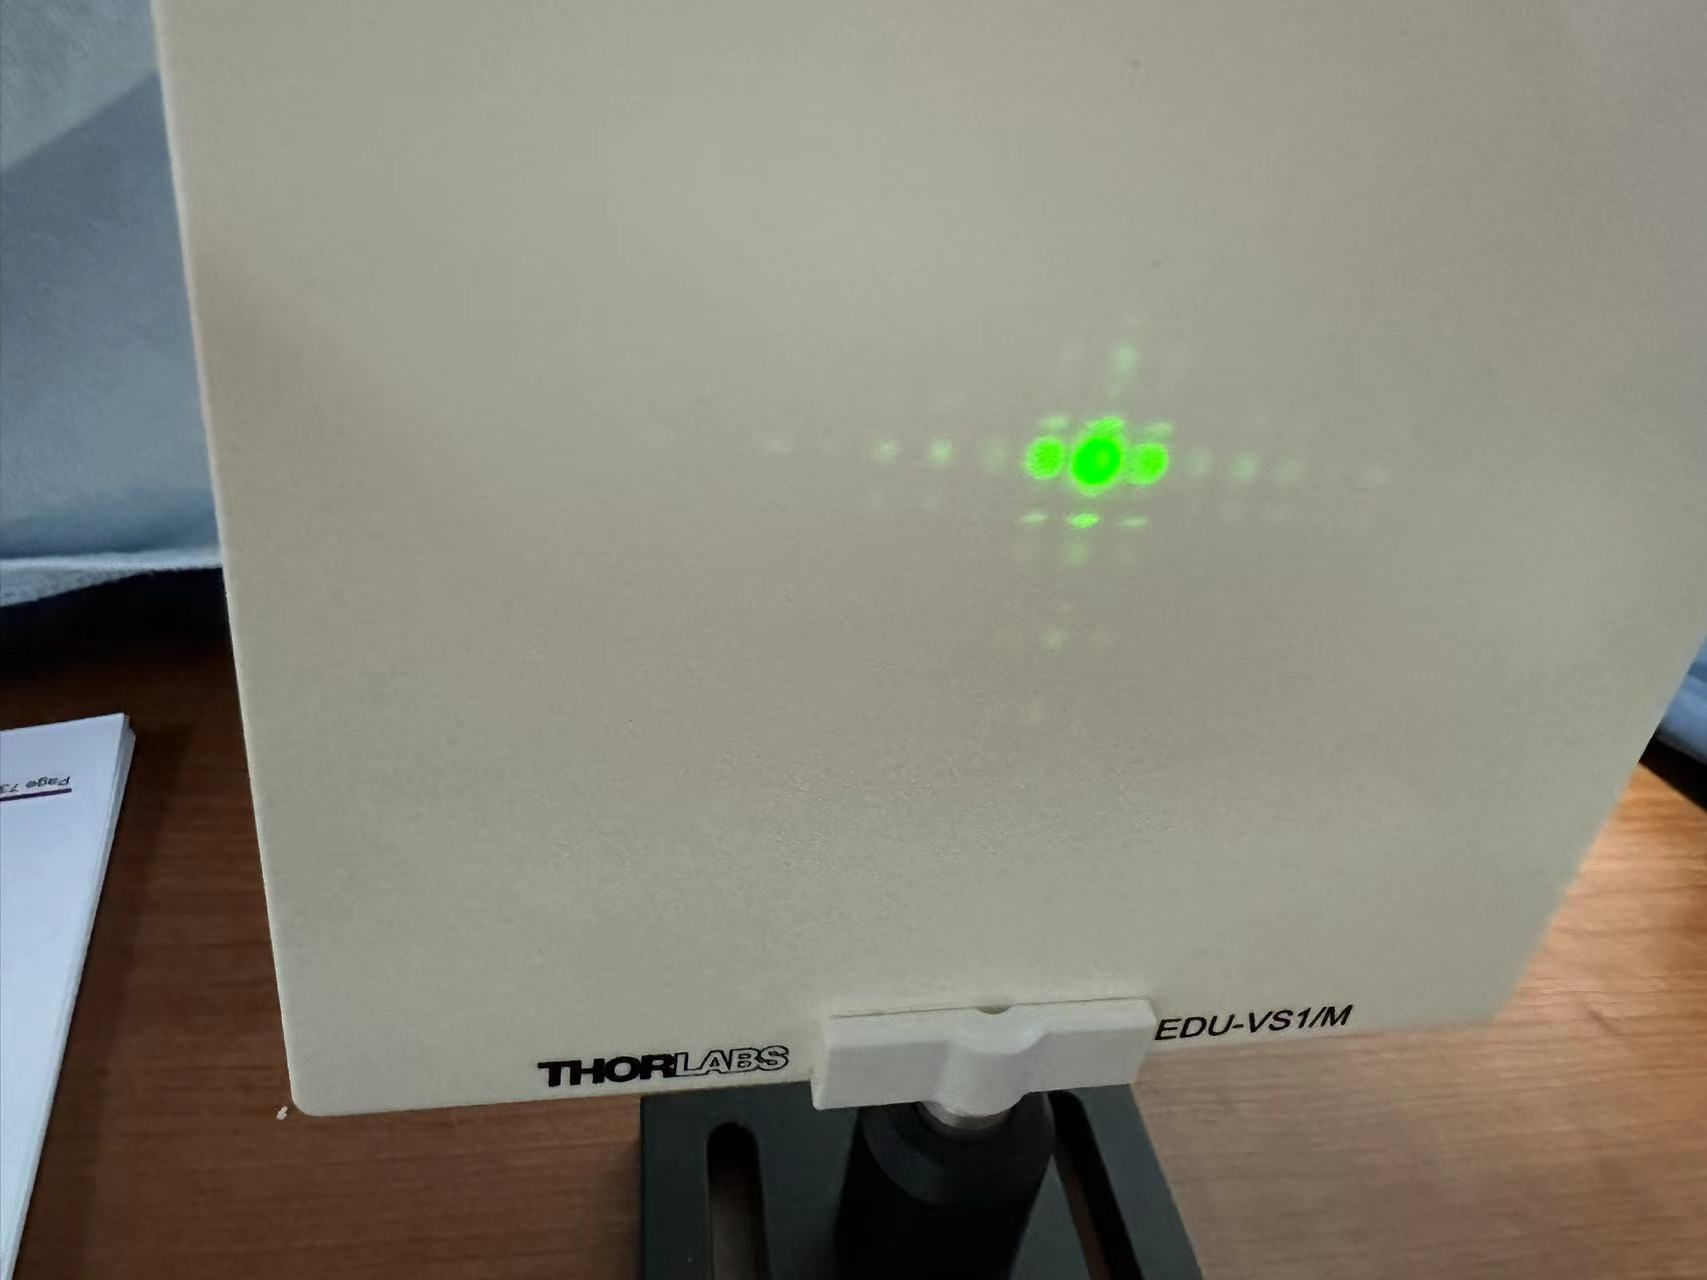
\includegraphics[width=\textwidth]{pictures/微信图片_20241010201051.jpg}
    \caption{F2 傅里叶面}
  \end{minipage}
  \hspace{0.1\textwidth} % 图片之间的水平间距
  \begin{minipage}[b]{0.3\textwidth}
    \centering
    
\includegraphics[width=\textwidth]{pictures/F2-mask-Ex8.png}
    \caption{F2 相机成像}
  \end{minipage}
\end{figure}

再用 VA100 作为 Mask,遮住傅里叶面上除了中间列以外的其他部分。观察到图像变为横条纹,这是因为有水平分量的波数均被滤去。
\begin{figure}[H]
  \centering
  \begin{minipage}[b]{0.2\textwidth}
    \centering
    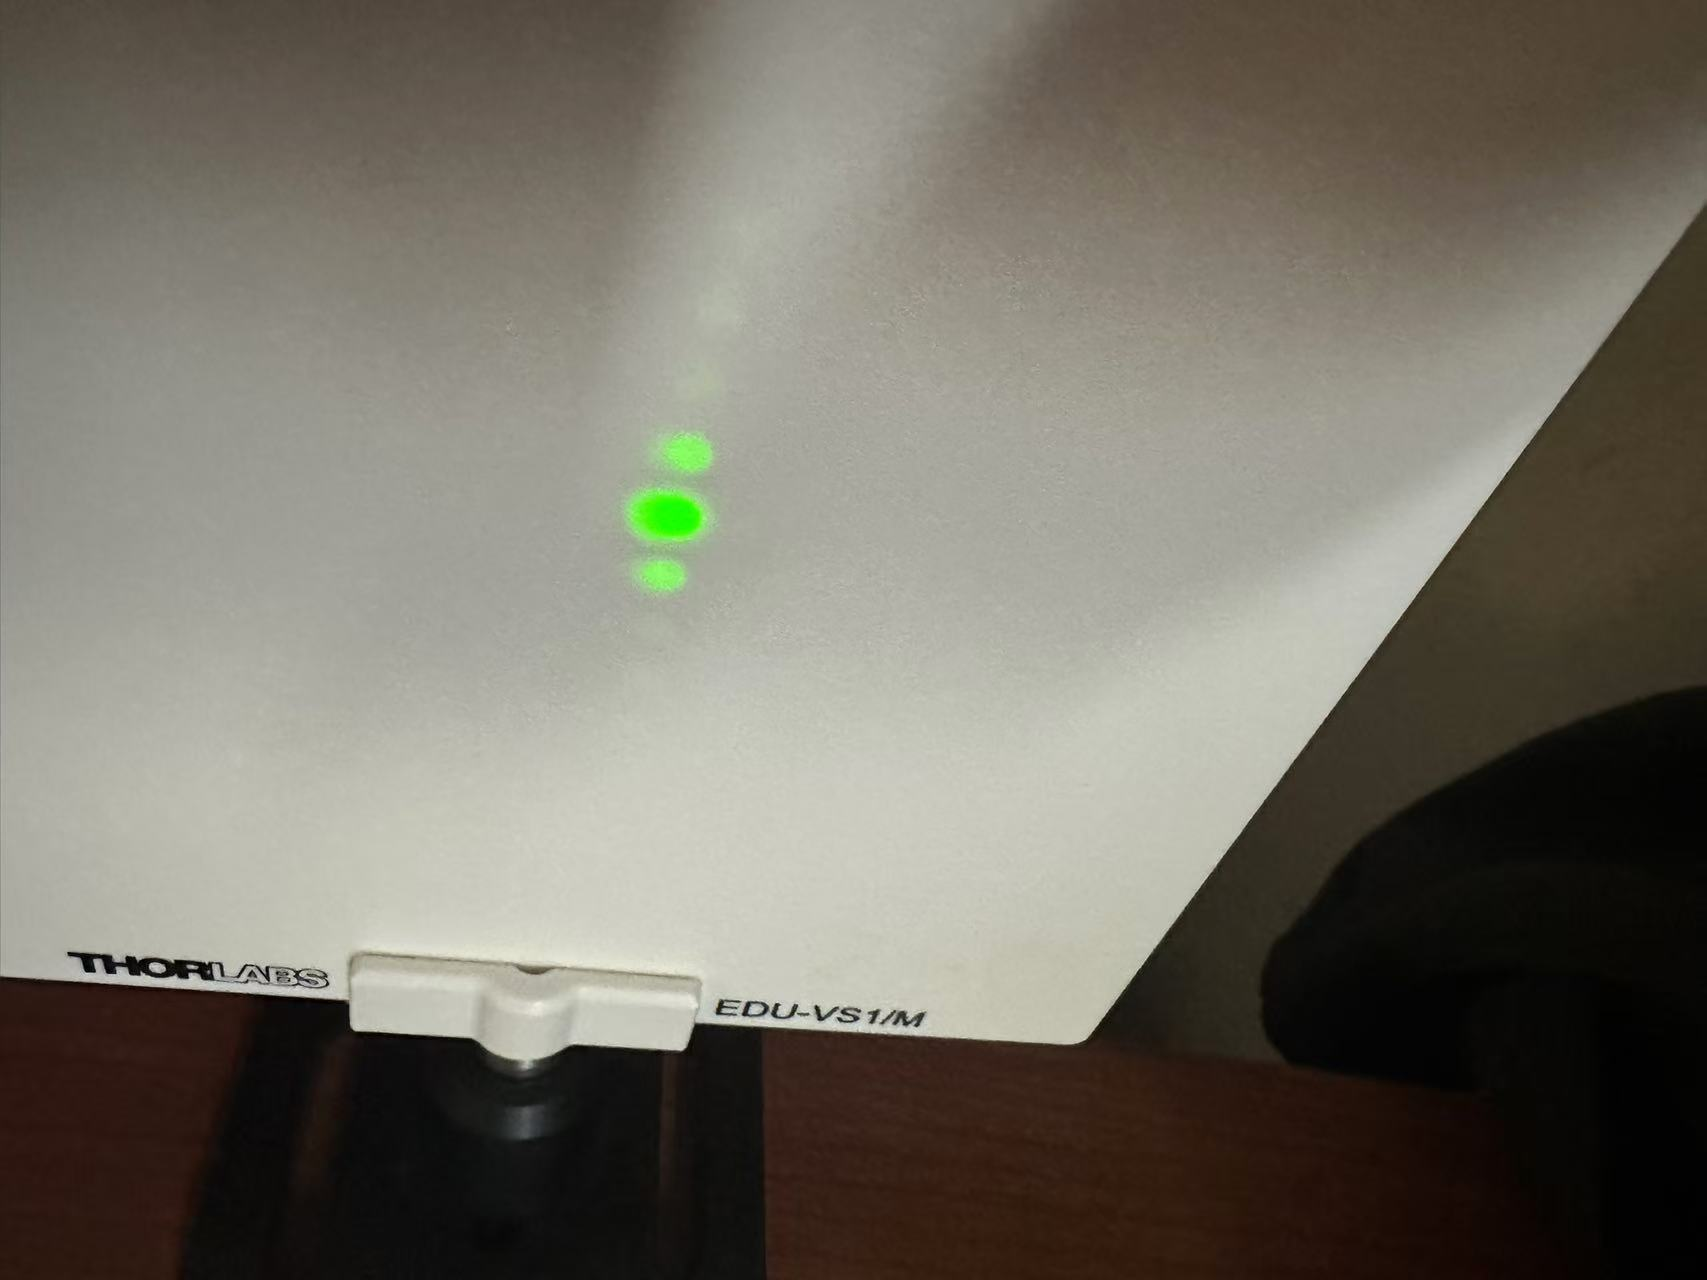
\includegraphics[width=\textwidth]{pictures/微信图片_20241017164802.jpg}
    \caption{F2 傅里叶面}
  \end{minipage}
  \hspace{0.1\textwidth} % 图片之间的水平间距
  \begin{minipage}[b]{0.3\textwidth}
    \centering
    
\includegraphics[width=\textwidth]{pictures/F2-mask-Ex9.png}
    \caption{F2 相机成像}
  \end{minipage}
\end{figure}
\subsubsection{F6}
调整 Target 上的 F6 图像到光路中,使其能够在相机中清晰成像,并观察屏上的傅里叶图像。
\begin{figure}[H]
  \centering
  \begin{minipage}[b]{0.2\textwidth}
    \centering
    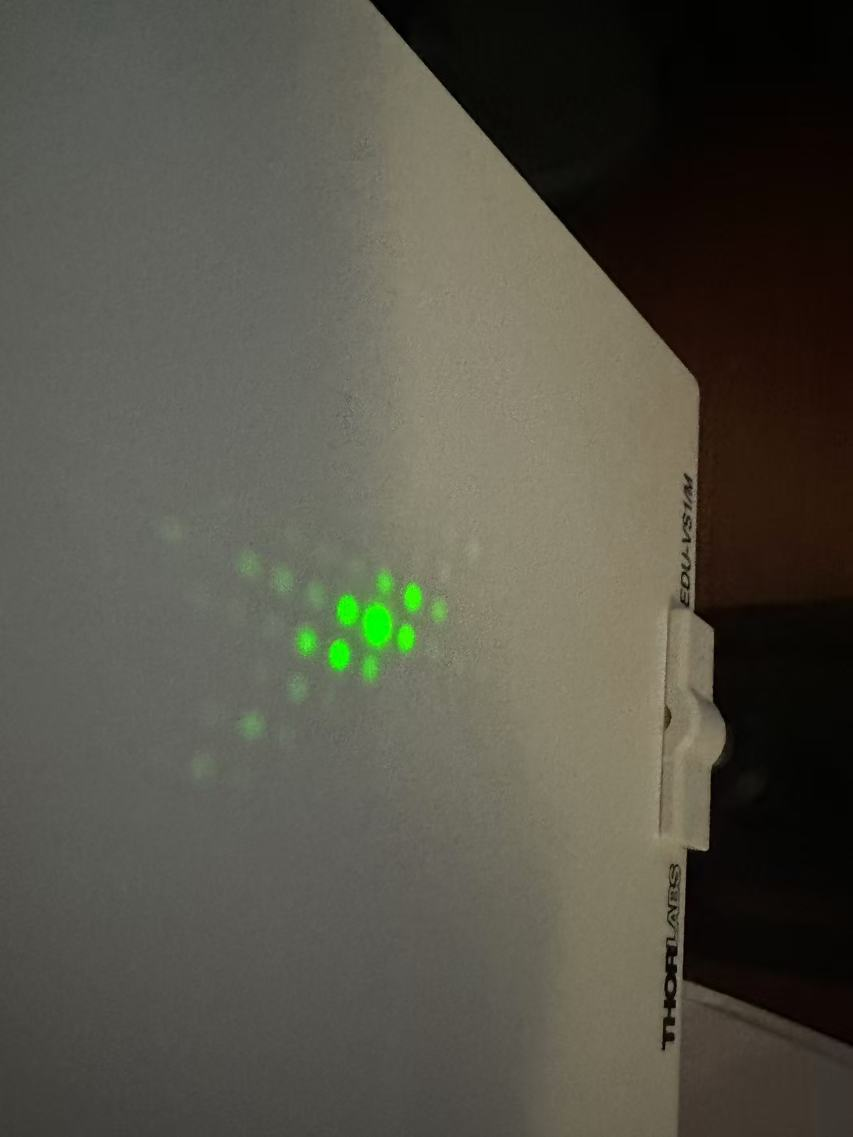
\includegraphics[width=\textwidth]{pictures/微信图片_20241017164805.jpg}
    \caption{F6 傅里叶面}
  \end{minipage}
  \hspace{0.1\textwidth} % 图片之间的水平间距
  \begin{minipage}[b]{0.3\textwidth}
    \centering
    
\includegraphics[width=\textwidth]{pictures/F6-nomask.png}
    \caption{F6 相机成像}
  \end{minipage}
\end{figure}

用 VA100 遮住傅里叶面上除了中间列以外的其他部分。观察到图像变为横条纹,这同样是因为具有水平分量的波数均被滤去。
\begin{figure}[H]
  \centering
  \begin{minipage}[b]{0.2\textwidth}
    \centering
    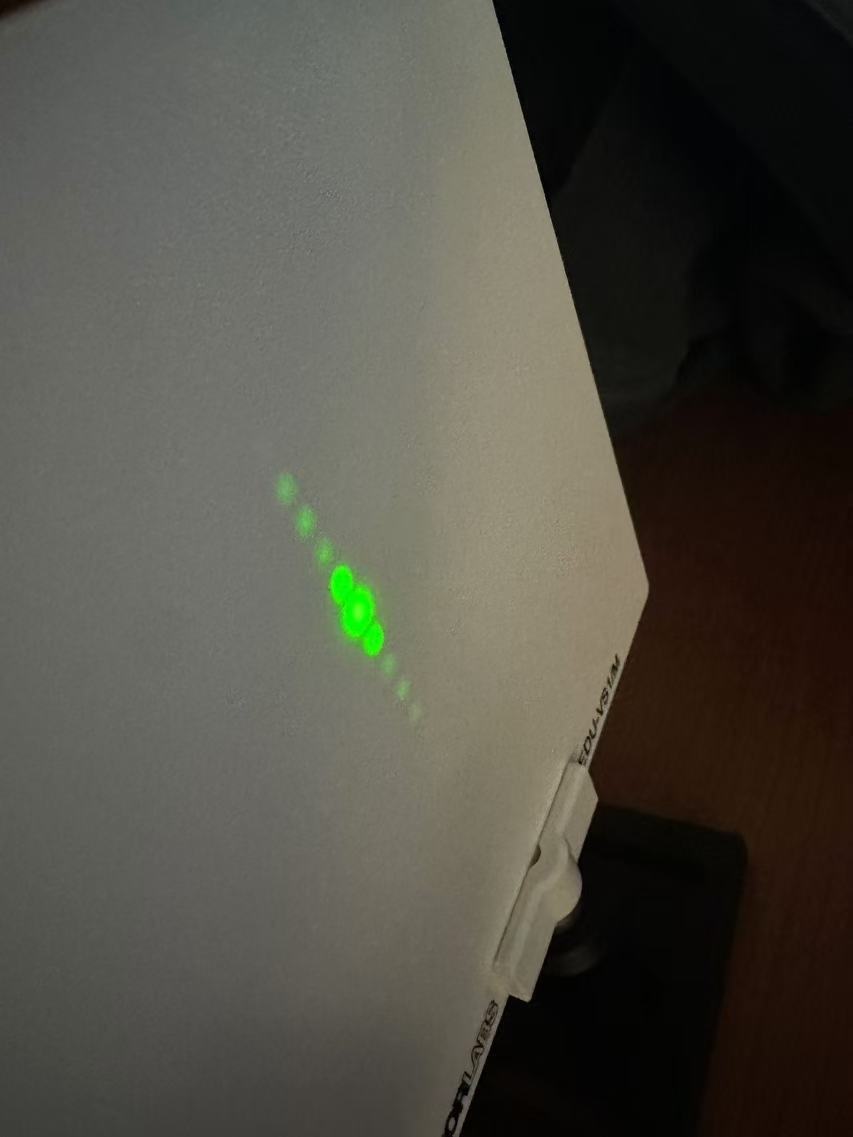
\includegraphics[width=\textwidth]{pictures/微信图片_20241017164808.jpg}
    \caption{F6 傅里叶面}
  \end{minipage}
  \hspace{0.1\textwidth} % 图片之间的水平间距
  \begin{minipage}[b]{0.3\textwidth}
    \centering
    
\includegraphics[width=\textwidth]{pictures/F6-mask-Ex11.png}
    \caption{F6 相机成像}
  \end{minipage}
\end{figure}
\subsubsection{F7}
调整 Target 上的 F7 图像到光路中,使其能够在相机中清晰成像。观察到傅里叶图像有多个从中心向外的射线,这是因为 F7 具有多个方向的平移不变性。
\begin{figure}[H]
  \centering
  \begin{minipage}[b]{0.2\textwidth}
    \centering
    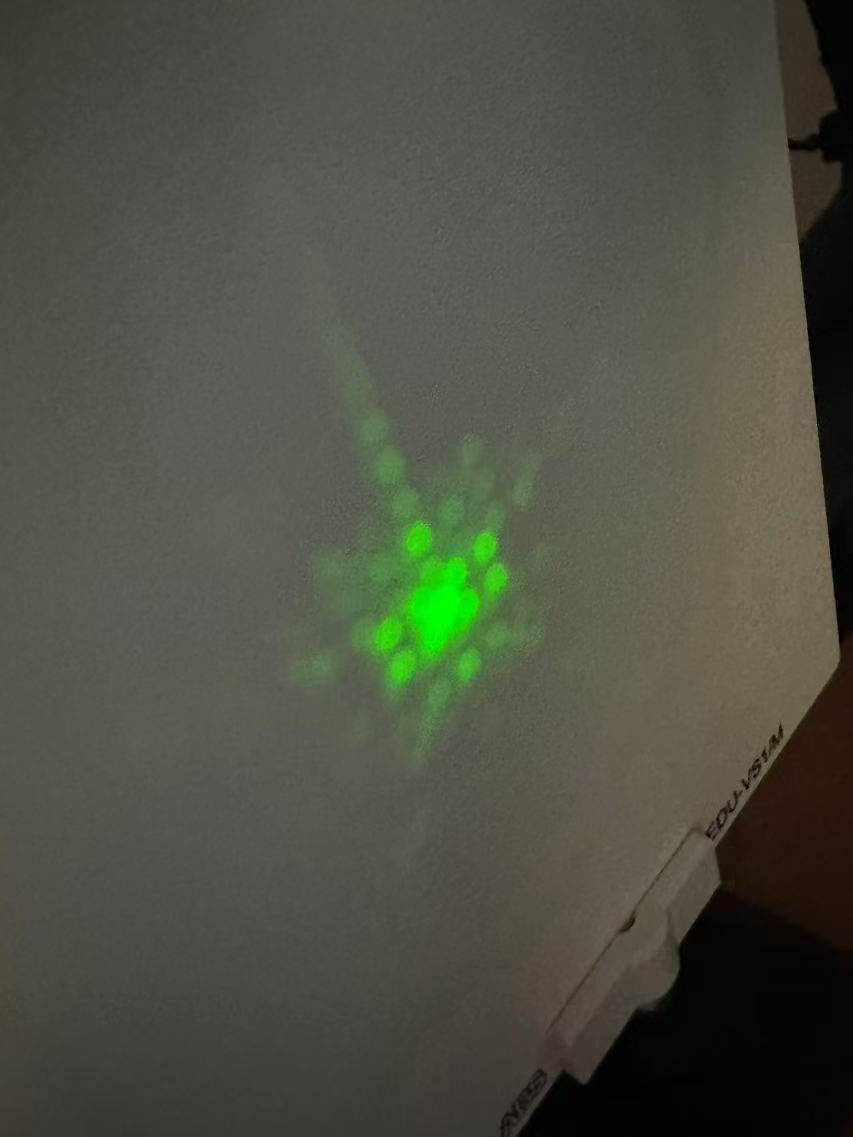
\includegraphics[width=\textwidth]{pictures/微信图片_20241017164811.jpg}
    \caption{F7 傅里叶面}
  \end{minipage}
  \hspace{0.1\textwidth} % 图片之间的水平间距
  \begin{minipage}[b]{0.3\textwidth}
    \centering
    
\includegraphics[width=\textwidth]{pictures/F7-nomask.png}
    \caption{F7 相机成像}
  \end{minipage}
\end{figure}

用 VA100 遮住傅里叶面上除了中间列以外的其他部分。观察到图像变为有深浅变化的厚横条纹,这是因为 F7 在竖直方向上有多种频率。
\begin{figure}[H]
  \centering
  \begin{minipage}[b]{0.2\textwidth}
    \centering
    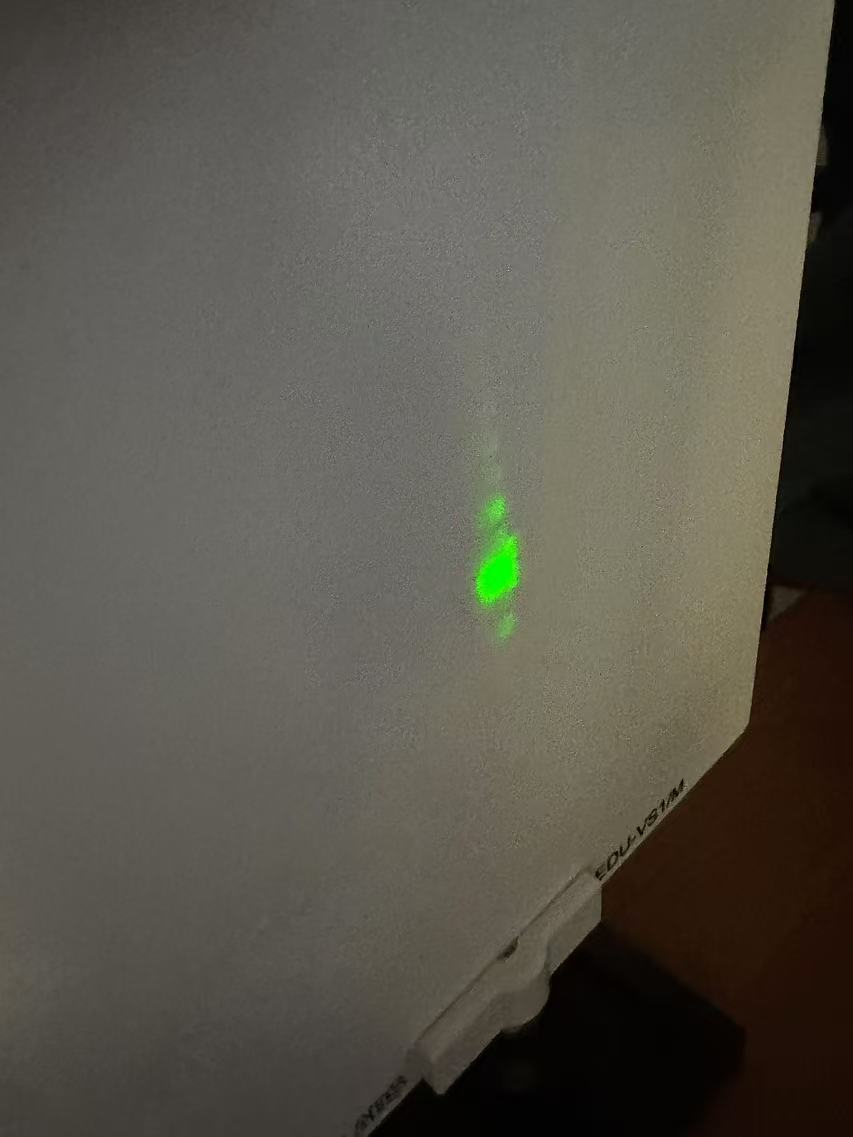
\includegraphics[width=\textwidth]{pictures/微信图片_20241017164815.jpg}
    \caption{F7 傅里叶面}
  \end{minipage}
  \hspace{0.1\textwidth} % 图片之间的水平间距
  \begin{minipage}[b]{0.3\textwidth}
    \centering
    
\includegraphics[width=\textwidth]{pictures/F7-mask-Ex12.png}
    \caption{F7 相机成像}
  \end{minipage}
\end{figure}
\subsubsection{F11}
调整 Target 上的 F11 图像到光路中,使其能够在相机中清晰成像,并观察屏上的傅里叶图像。
\begin{figure}[H]
  \centering
  \begin{minipage}[b]{0.2\textwidth}
    \centering
    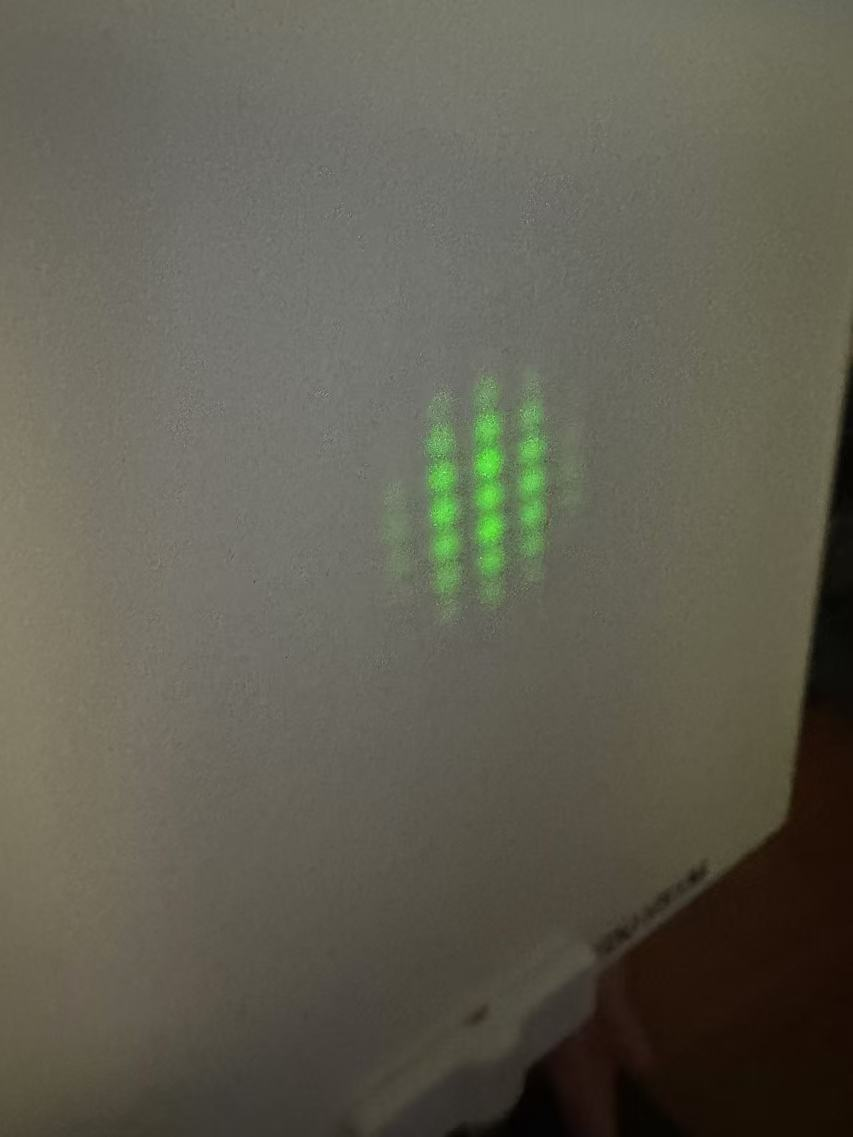
\includegraphics[width=\textwidth]{pictures/微信图片_20241017164819.jpg}
    \caption{F11 傅里叶面}
  \end{minipage}
  \hspace{0.1\textwidth} % 图片之间的水平间距
  \begin{minipage}[b]{0.3\textwidth}
    \centering
    
\includegraphics[width=\textwidth]{pictures/F11-nomask.png}
    \caption{F11 相机成像}
  \end{minipage}
\end{figure}

用 VA100 遮住傅里叶面上除了中间列以外的其他部分。观察到图像变为稀疏的细横条纹,这是因为 F11 原本在竖直方向上就是稀疏的。
\begin{figure}[H]
  \centering
  \begin{minipage}[b]{0.2\textwidth}
    \centering
    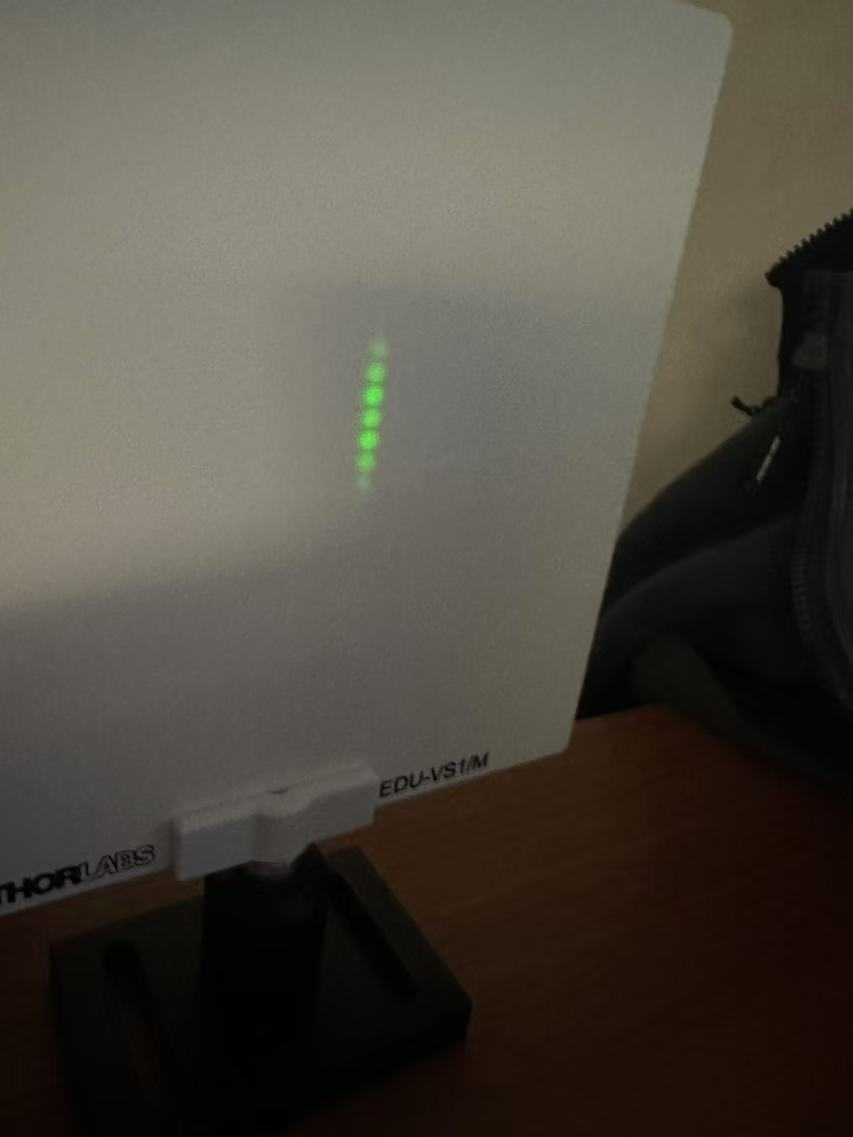
\includegraphics[width=\textwidth]{pictures/微信图片_20241017164822.jpg}
    \caption{F11 傅里叶面}
  \end{minipage}
  \hspace{0.1\textwidth} % 图片之间的水平间距
  \begin{minipage}[b]{0.3\textwidth}
    \centering
    
\includegraphics[width=\textwidth]{pictures/F11-mask-Ex13.png}
    \caption{F11 相机成像}
  \end{minipage}
\end{figure}
\subsubsection{F9}
调整 Target 上的 F9 图像到光路中,使其能够在相机中清晰成像。观察到傅里叶图像仅有水平光点,这是因为 F9 是由竖条纹构成的,其主要的波数均是水平方向的。
\begin{figure}[H]
  \centering
  \begin{minipage}[b]{0.2\textwidth}
    \centering
    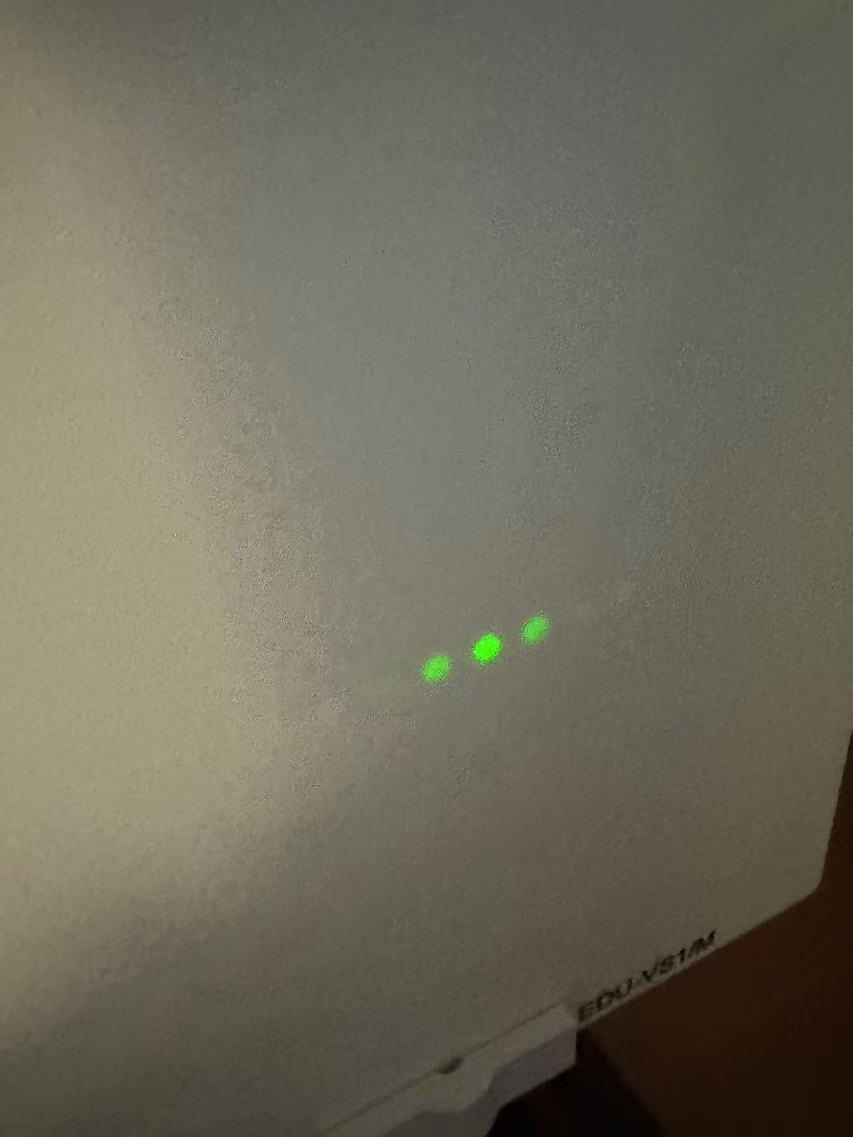
\includegraphics[width=\textwidth]{pictures/微信图片_20241017164825.jpg}
    \caption{F9 傅里叶面}
  \end{minipage}
  \hspace{0.1\textwidth} % 图片之间的水平间距
  \begin{minipage}[b]{0.3\textwidth}
    \centering
    
\includegraphics[width=\textwidth]{pictures/F9-nomask.png}
    \caption{F9 相机成像}
  \end{minipage}
\end{figure}

用 VA100 遮住傅里叶面上除了零级以外的其他部分。观察到没有竖条纹的笑脸,这是由于在水平方向上周期性变化的成分均被滤去。
\begin{figure}[H]
  \centering
  \begin{minipage}[b]{0.2\textwidth}
    \centering
    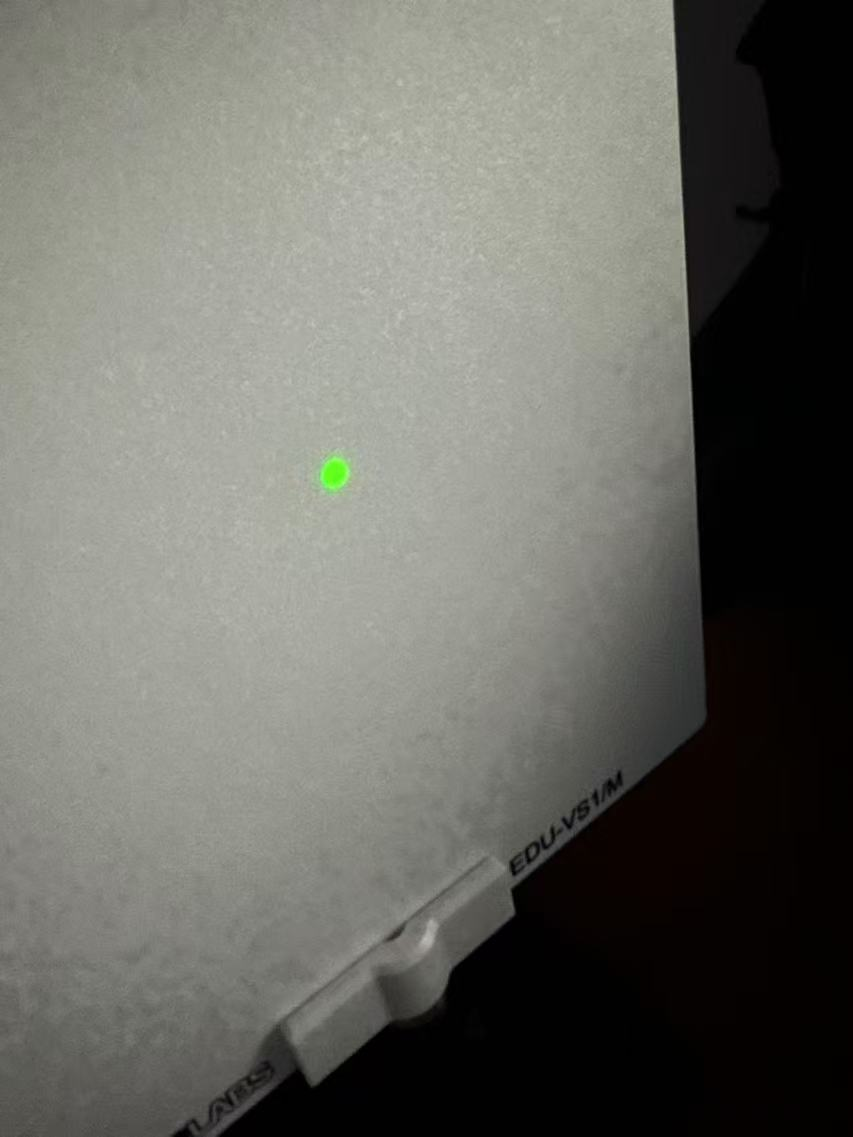
\includegraphics[width=\textwidth]{pictures/微信图片_20241017164828.jpg}
    \caption{F9 傅里叶面}
  \end{minipage}
  \hspace{0.1\textwidth} % 图片之间的水平间距
  \begin{minipage}[b]{0.3\textwidth}
    \centering
    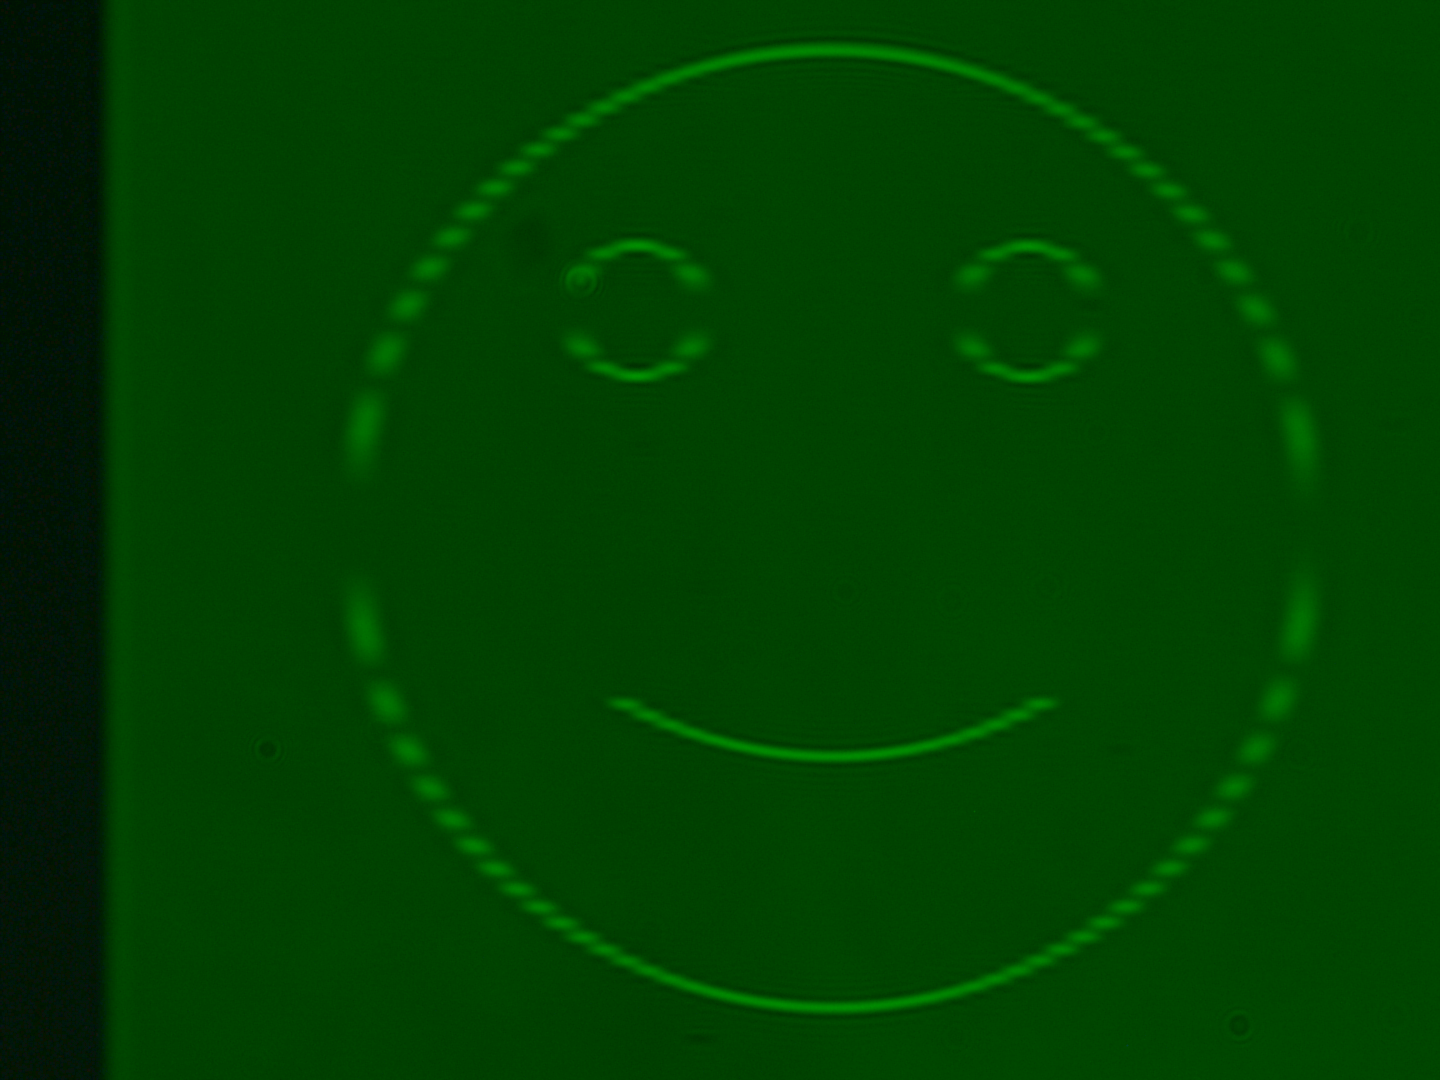
\includegraphics[width=\textwidth]{pictures/F9-mask-Ex14.png}
    \caption{F9 相机成像}
  \end{minipage}
\end{figure}

用 VA100 分别仅保留傅里叶面上的一级和二级。均能在相机中观察到笑脸。
\begin{figure}[H]
  \centering
  \begin{minipage}[b]{0.3\textwidth}
    \centering
    
\includegraphics[width=\textwidth]{pictures/F9-mask1-Ex16.png}
    \caption{F9 相机成像(保留一级)}
  \end{minipage}
  \hspace{0.1\textwidth} % 图片之间的水平间距
  \begin{minipage}[b]{0.3\textwidth}
    \centering
    
\includegraphics[width=\textwidth]{pictures/F9-mask2-Ex16.png}
    \caption{F9 相机成像(保留二级)}
  \end{minipage}
\end{figure}
\subsubsection{F12}
调整 Target 上的 F12 图像到光路中,使其能够在相机中清晰成像,并观察屏上的傅里叶图像。
\begin{figure}[H]
  \centering
  \begin{minipage}[b]{0.2\textwidth}
    \centering
    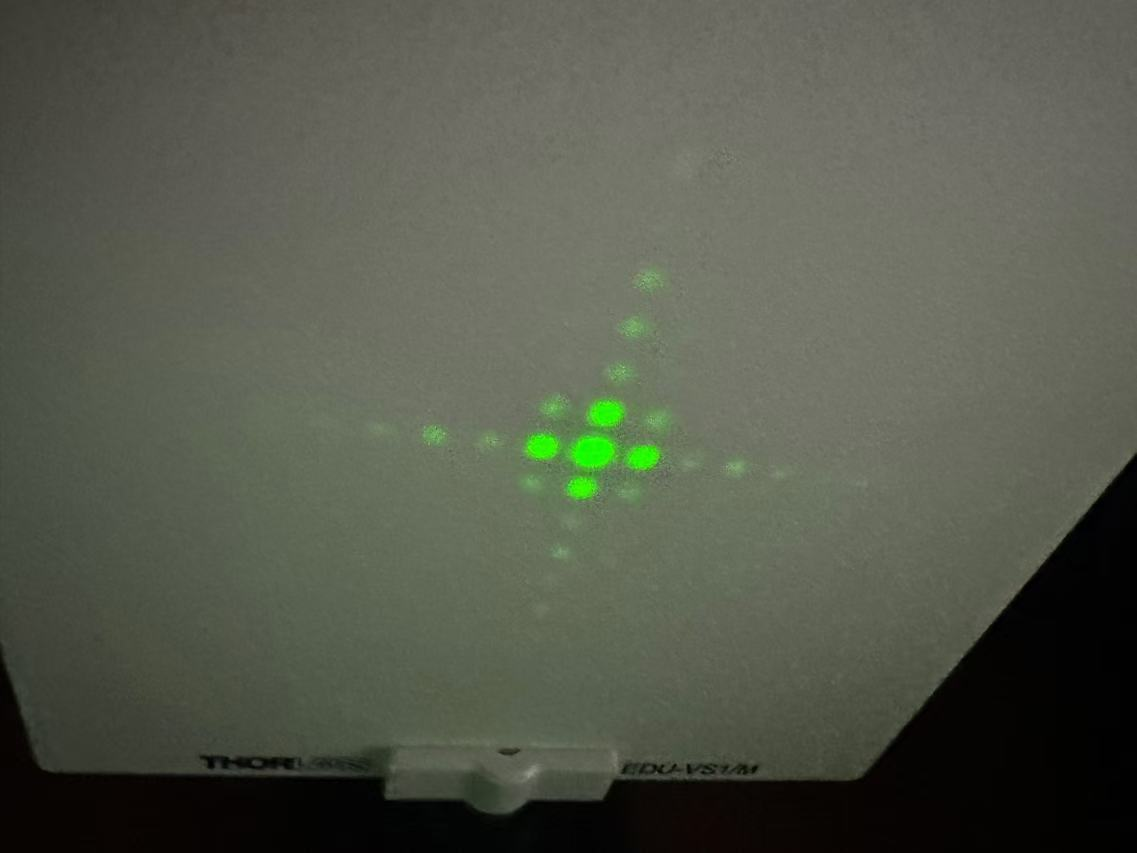
\includegraphics[width=\textwidth]{pictures/微信图片_20241017164831.jpg}
    \caption{F12 傅里叶面}
  \end{minipage}
  \hspace{0.1\textwidth} % 图片之间的水平间距
  \begin{minipage}[b]{0.3\textwidth}
    \centering
    
\includegraphics[width=\textwidth]{pictures/F12-nomask.png}
    \caption{F12 相机成像}
  \end{minipage}
\end{figure}

用 VA100 遮住傅里叶面上除了中间列以外的其他部分。观察到 B 变暗而 A 亮度保持,这是因为 B 是水平周期条纹构成的,而 A 是竖直周期条纹构成的。
\begin{figure}[H]
  \centering
  \begin{minipage}[b]{0.2\textwidth}
    \centering
    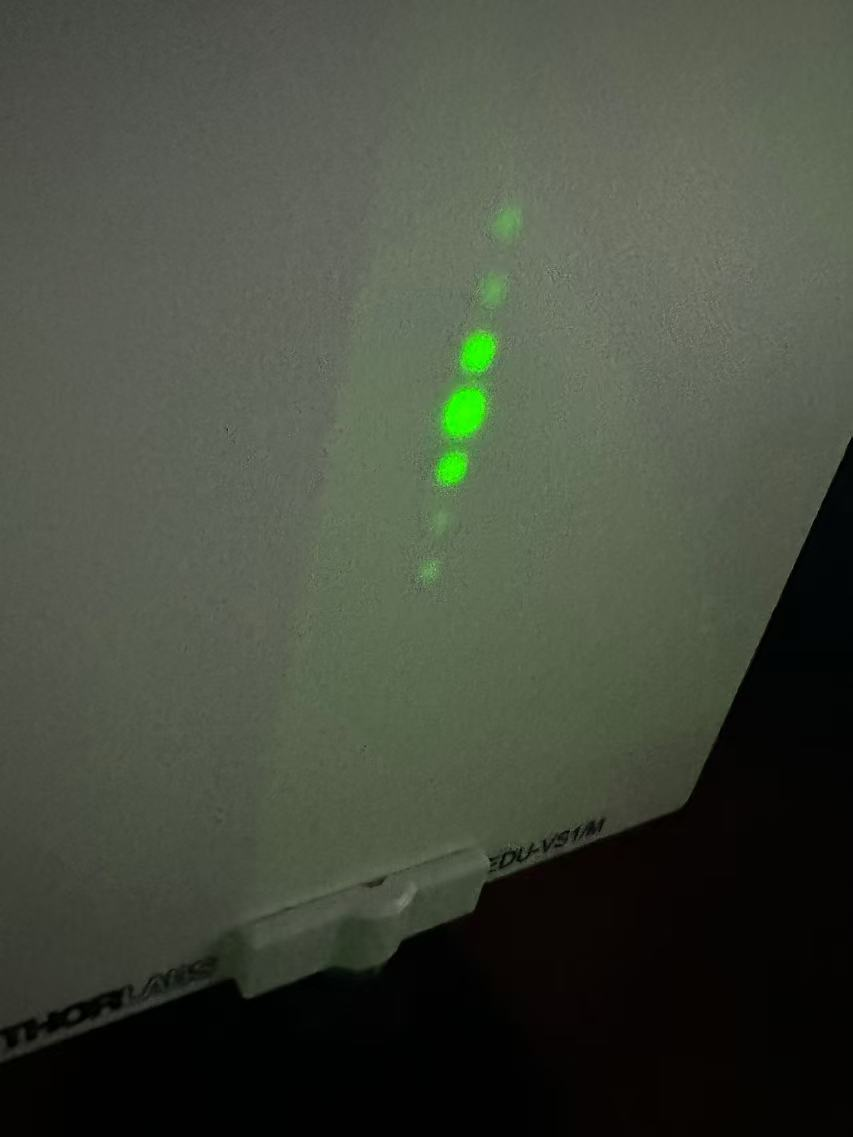
\includegraphics[width=\textwidth]{pictures/微信图片_20241017164835.jpg}
    \caption{F12 傅里叶面}
  \end{minipage}
  \hspace{0.1\textwidth} % 图片之间的水平间距
  \begin{minipage}[b]{0.3\textwidth}
    \centering
    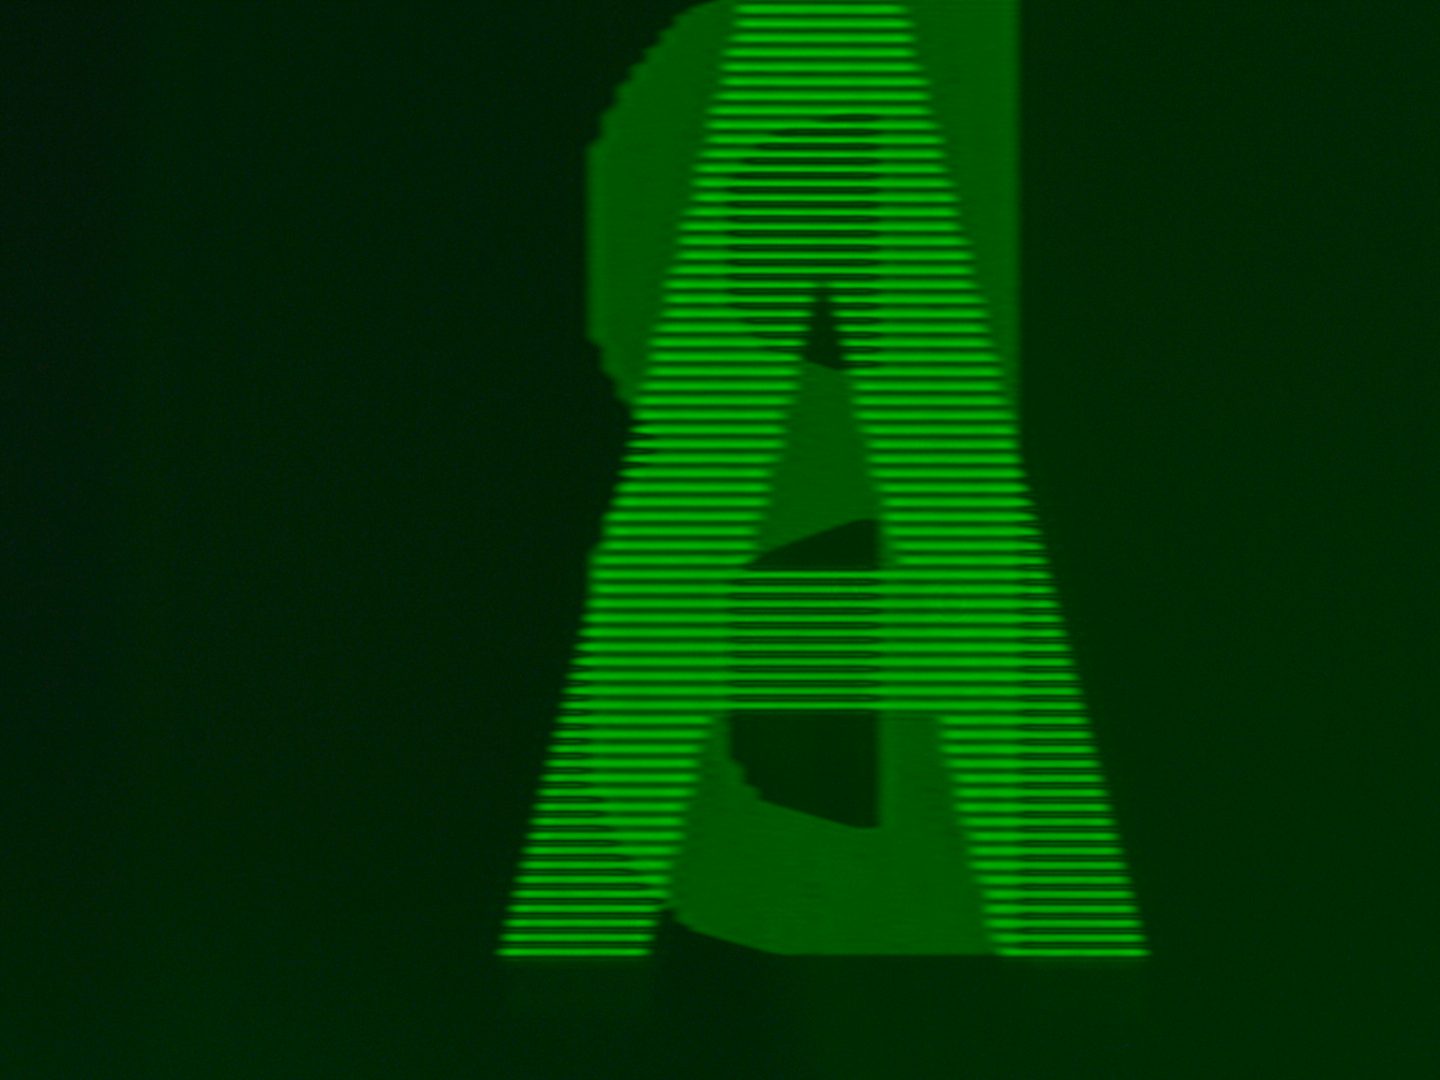
\includegraphics[width=\textwidth]{pictures/F12-mask-Ex17.png}
    \caption{F12 相机成像}
  \end{minipage}
\end{figure}
\subsubsection{F10}
调整 Target 上的 F10 图像到光路中,使其能够在相机中清晰成像,并观察屏上的傅里叶图像。
\begin{figure}[H]
  \centering
  \begin{minipage}[b]{0.2\textwidth}
    \centering
    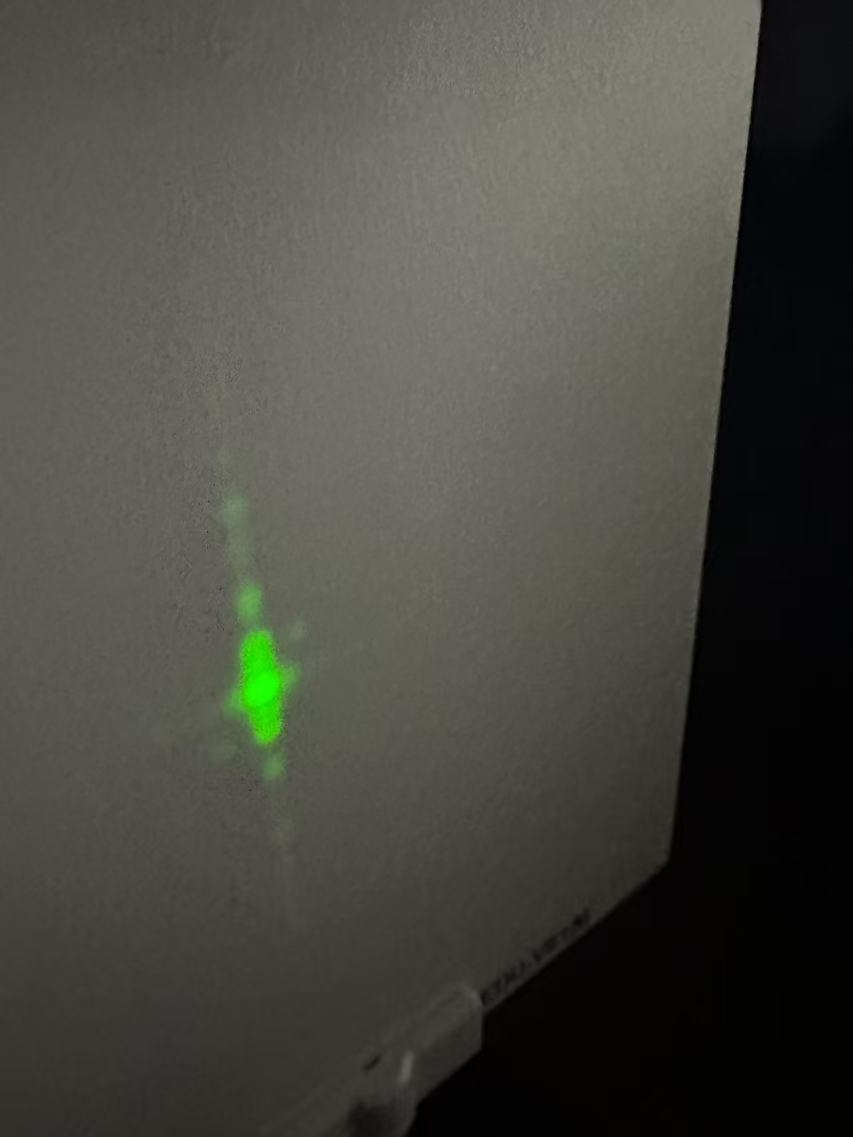
\includegraphics[width=\textwidth]{pictures/微信图片_20241017164838.jpg}
    \caption{F10 傅里叶面}
  \end{minipage}
  \hspace{0.1\textwidth} % 图片之间的水平间距
  \begin{minipage}[b]{0.3\textwidth}
    \centering
    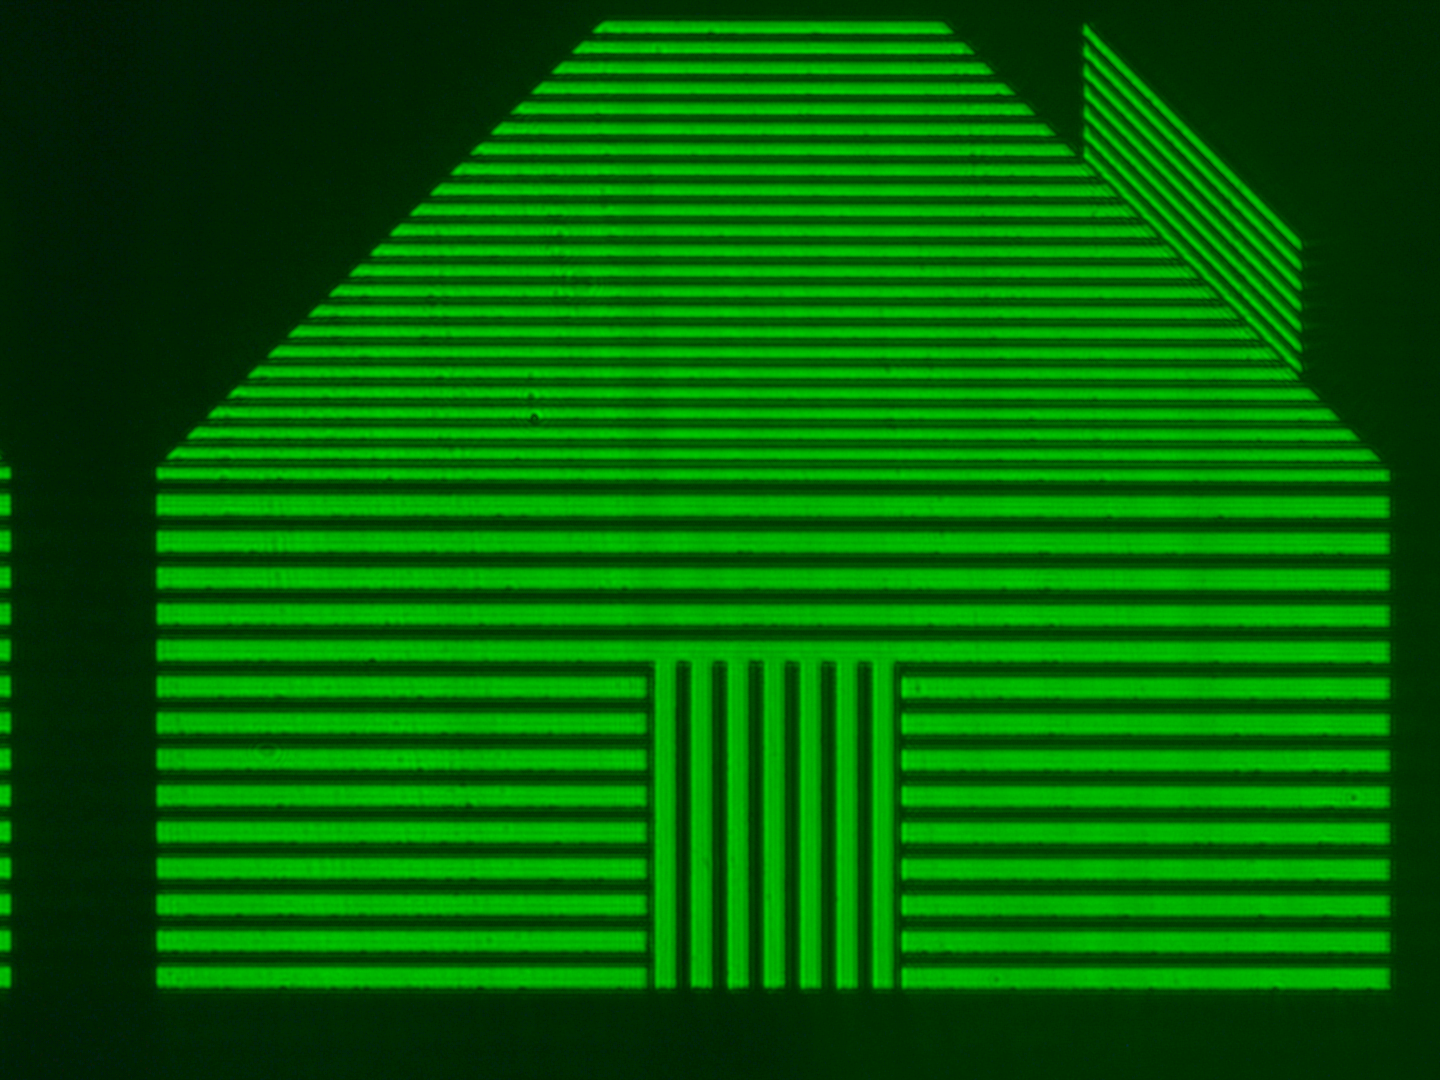
\includegraphics[width=\textwidth]{pictures/F10-nomask.png}
    \caption{F10 相机成像}
  \end{minipage}
\end{figure}

用 VA100 遮住傅里叶面上除了中间列以外的其他部分。观察到门和烟囱变暗而房子主体亮度保持,这是因为门和烟囱分别是斜条纹和竖条纹,因此被滤去,而房子主题是横条纹故没有被滤掉。
\begin{figure}[H]
  \centering
  \begin{minipage}[b]{0.2\textwidth}
    \centering
    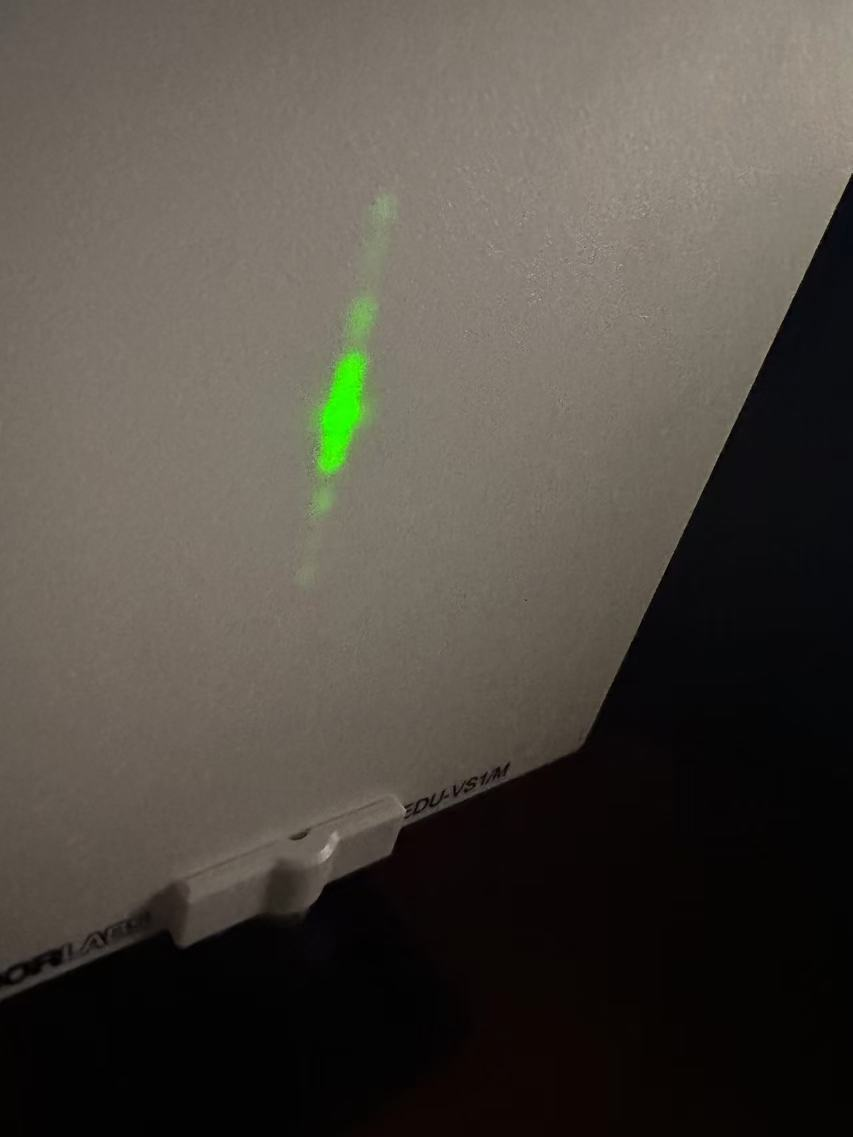
\includegraphics[width=\textwidth]{pictures/微信图片_20241017164842.jpg}
    \caption{F10 傅里叶面}
  \end{minipage}
  \hspace{0.1\textwidth} % 图片之间的水平间距
  \begin{minipage}[b]{0.3\textwidth}
    \centering
    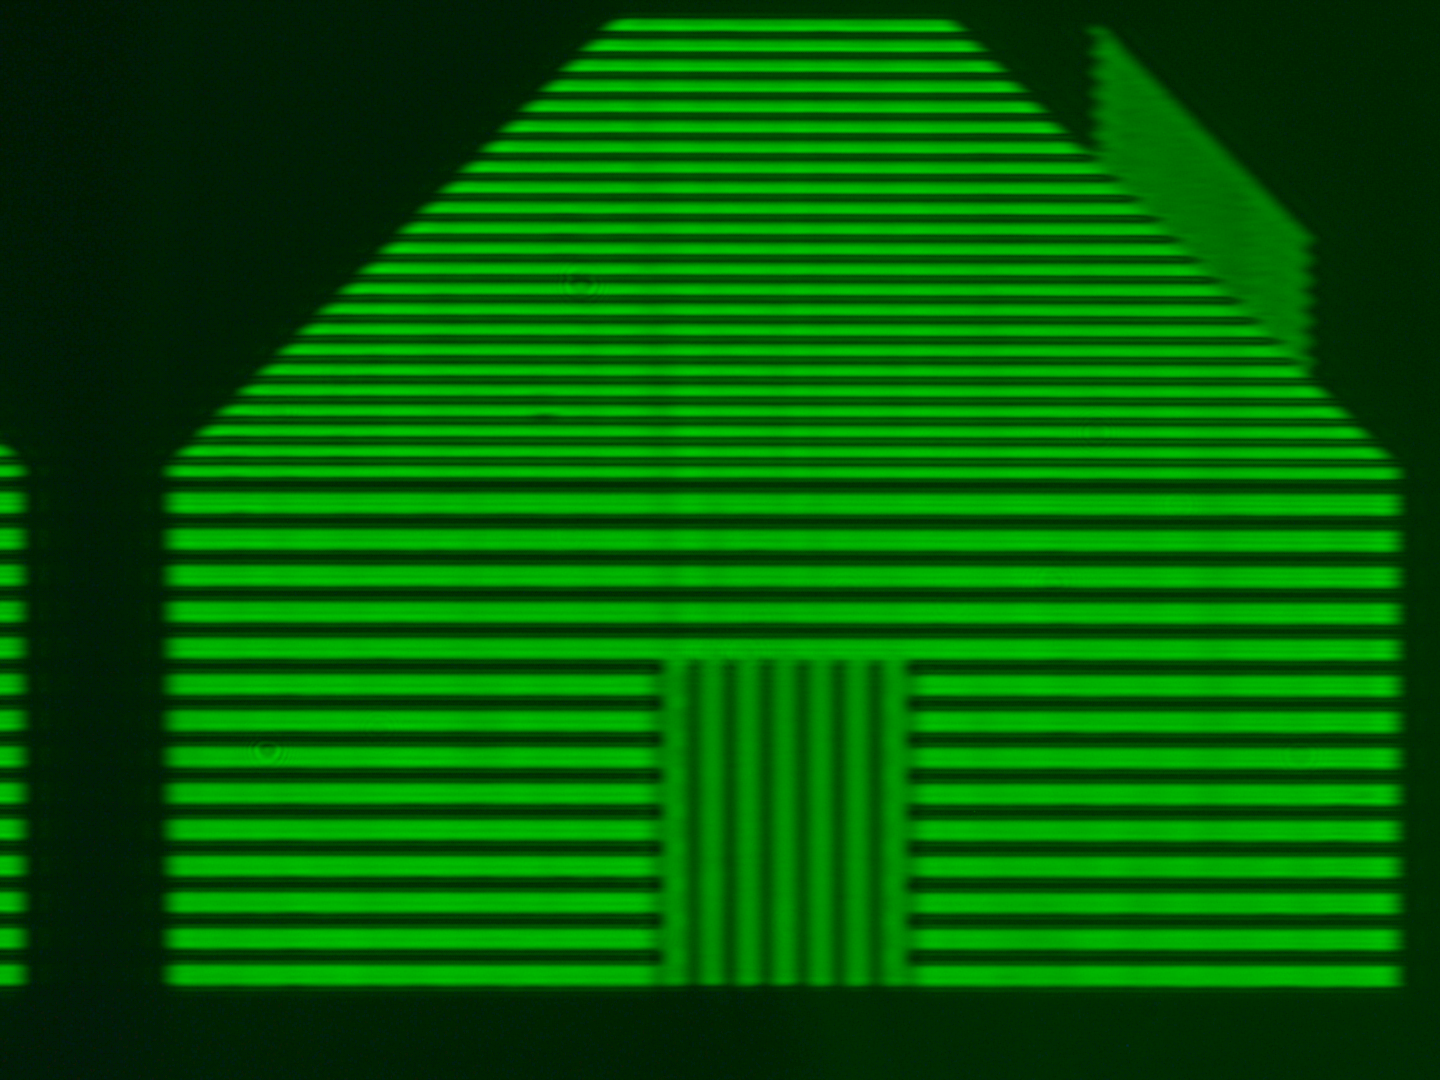
\includegraphics[width=\textwidth]{pictures/F10-mask-Ex19.png}
    \caption{F10 相机成像}
  \end{minipage}
\end{figure}
\subsubsection{F8}
调整 Target 上的 F8 图像到光路中,使其能够在相机中清晰成像,并观察屏上的傅里叶图像。
\begin{figure}[H]
  \centering
  \begin{minipage}[b]{0.2\textwidth}
    \centering
    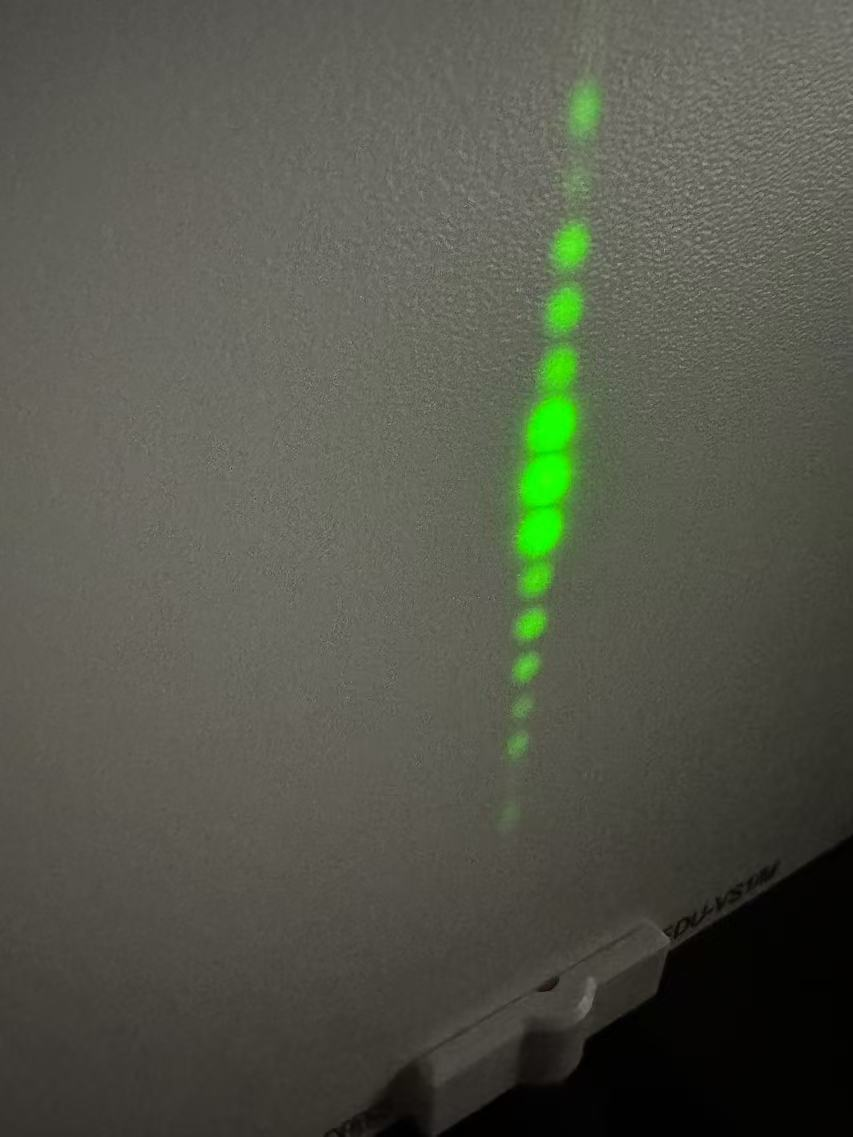
\includegraphics[width=\textwidth]{pictures/微信图片_20241017164844.jpg}
    \caption{F8 傅里叶面}
  \end{minipage}
  \hspace{0.1\textwidth} % 图片之间的水平间距
  \begin{minipage}[b]{0.3\textwidth}
    \centering
    
\includegraphics[width=\textwidth]{pictures/F8-nomask.png}
    \caption{F8 相机成像}
  \end{minipage}
\end{figure}

将 EDU-TGC1 作为 Mask,用横条纹遮住傅里叶面上的奇数级。观察到图像横条纹变密集,这是因为仅保留偶数级后图像在空间上的基频变为原本的两倍。
\begin{figure}[H]
  \centering
  \begin{minipage}[b]{0.2\textwidth}
    \centering
    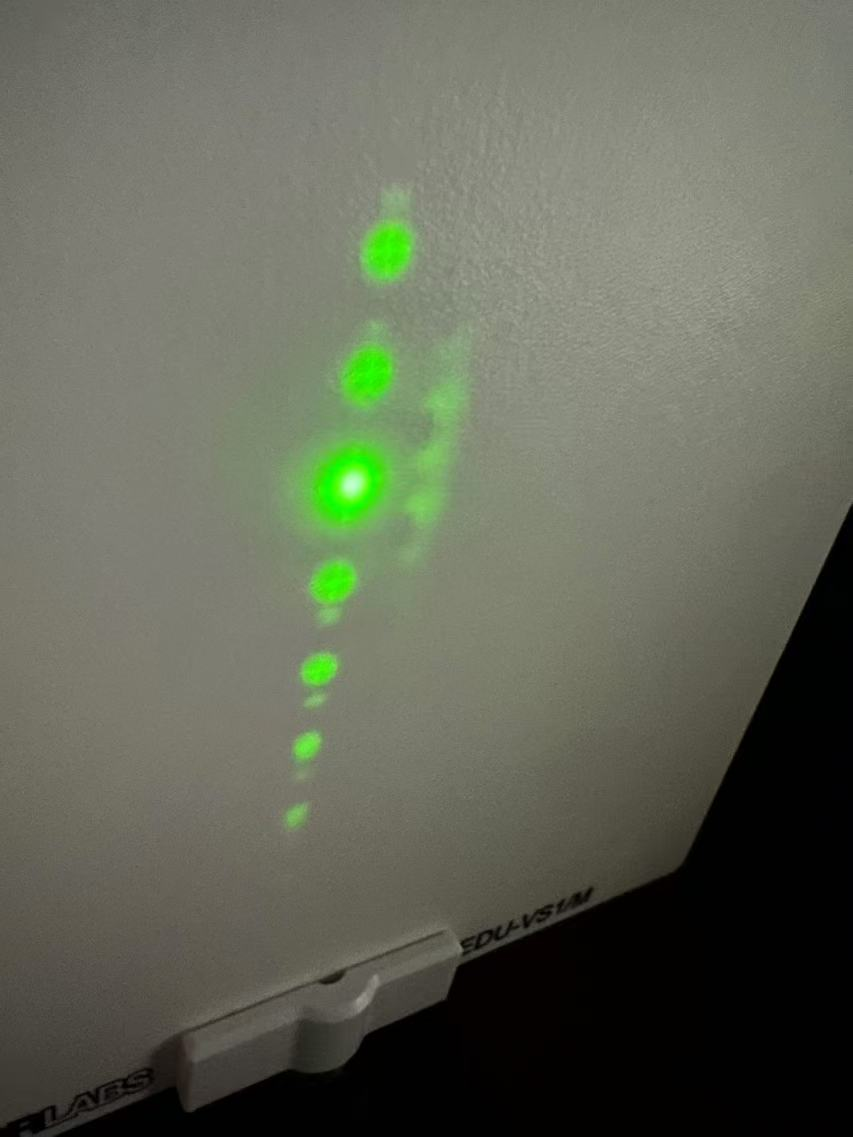
\includegraphics[width=\textwidth]{pictures/微信图片_20241017164851.jpg}
    \caption{F8 傅里叶面}
  \end{minipage}
  \hspace{0.1\textwidth} % 图片之间的水平间距
  \begin{minipage}[b]{0.3\textwidth}
    \centering
    
\includegraphics[width=\textwidth]{pictures/F8-mask-Ex20.png}
    \caption{F8 相机成像}
  \end{minipage}
\end{figure}
\subsubsection{F5}
调整 Target 上的 F5 图像到光路中,使其能够在相机中清晰成像。观察到傅里叶图像有六个方向的射线,这是因为 F5 在这些方向上均有平移对称性。
\begin{figure}[H]
  \centering
  \begin{minipage}[b]{0.2\textwidth}
    \centering
    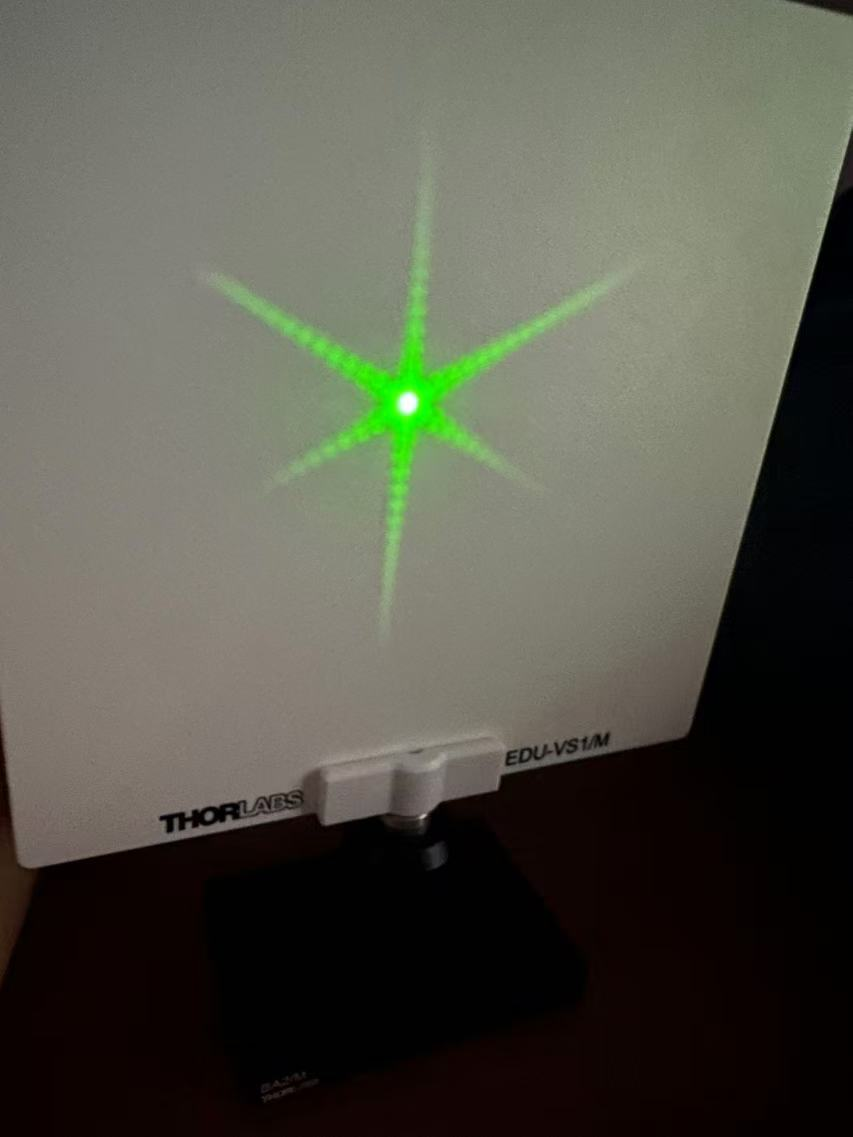
\includegraphics[width=\textwidth]{pictures/微信图片_20241017164855.jpg}
    \caption{F5 傅里叶面}
  \end{minipage}
  \hspace{0.1\textwidth} % 图片之间的水平间距
  \begin{minipage}[b]{0.3\textwidth}
    \centering
    
\includegraphics[width=\textwidth]{pictures/F5-nomask.png}
    \caption{F5 相机成像}
  \end{minipage}
\end{figure}

用 EDU-TGC1 遮住傅里叶面上各个方向的奇数级。观察到图像变为更密集排列的小三角形,这是因为空间基频变为原来的两倍。
\begin{figure}[H]
  \centering
  \begin{minipage}[b]{0.2\textwidth}
    \centering
    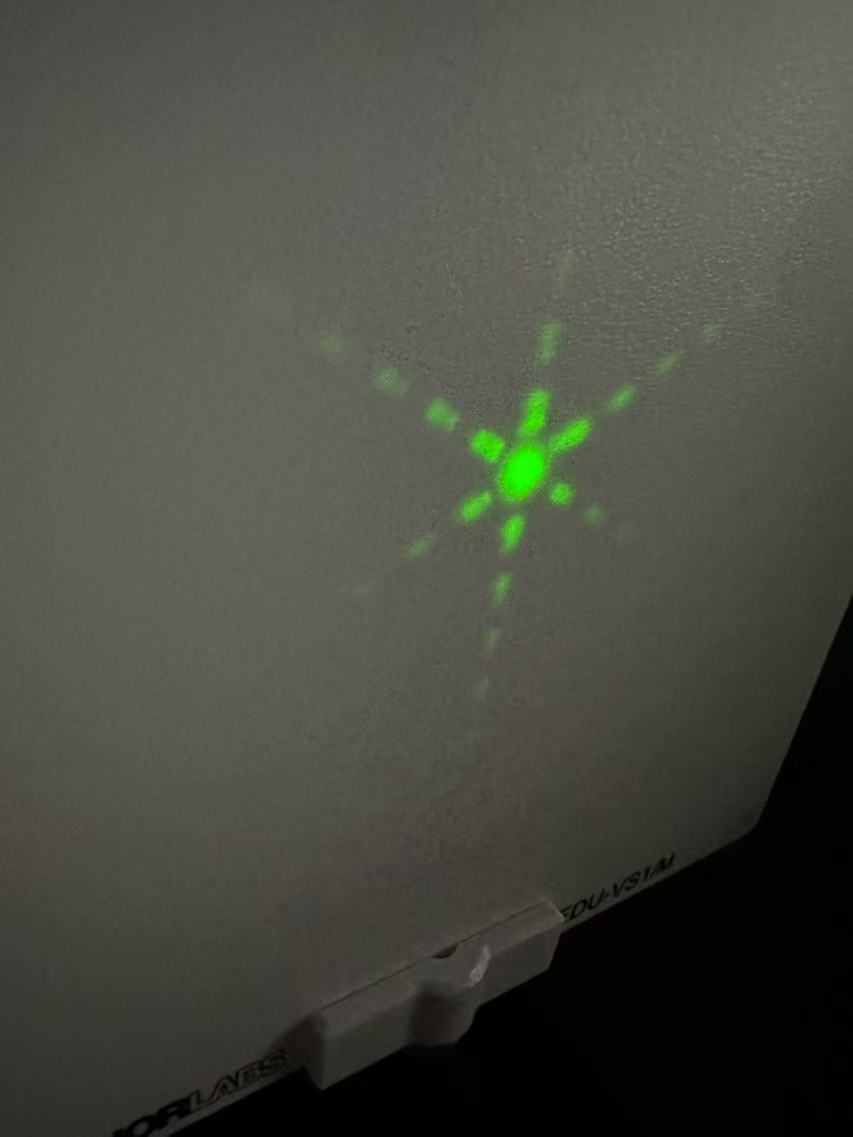
\includegraphics[width=\textwidth]{pictures/微信图片_20241017164858.jpg}
    \caption{F5 傅里叶面}
  \end{minipage}
  \hspace{0.1\textwidth} % 图片之间的水平间距
  \begin{minipage}[b]{0.3\textwidth}
    \centering
    
\includegraphics[width=\textwidth]{pictures/F5-mask-Ex21.png}
    \caption{F5 相机成像}
  \end{minipage}
\end{figure}
\subsubsection{F14}
调整 Target 上的 F14 图像到光路中,使其能够在相机中清晰成像,并观察屏上的傅里叶图像。
\begin{figure}[H]
  \centering
  \begin{minipage}[b]{0.2\textwidth}
    \centering
    \includegraphics[width=\textwidth]{pictures/微信图片_20241017164902.jpg}
    \caption{F14 傅里叶面}
  \end{minipage}
  \hspace{0.1\textwidth} % 图片之间的水平间距
  \begin{minipage}[b]{0.3\textwidth}
    \centering
    \includegraphics[width=\textwidth]{pictures/F14-nomask.png}
    \caption{F14 相机成像}
  \end{minipage}
\end{figure}

将 ID12(/M) 作为 Mask,缩小傅里叶面上可以通过的光圈大小。观察到图像中心周边变暗。
\begin{figure}[H]
  \centering
  \begin{minipage}[b]{0.2\textwidth}
    \centering
    \includegraphics[width=\textwidth]{pictures/微信图片_20241017164905.jpg}
    \caption{F14 傅里叶面}
  \end{minipage}
  \hspace{0.1\textwidth} % 图片之间的水平间距
  \begin{minipage}[b]{0.3\textwidth}
    \centering
    \includegraphics[width=\textwidth]{pictures/F14-mask1-Ex22.png}
    \caption{F14 相机成像}
  \end{minipage}
\end{figure}

再进一步缩小傅里叶面上可以通过的光圈大小到最小,观察到图像中心周边更大范围变暗。这是由于高频部分被滤去了更多,靠近图像中心的高频部分亮度变暗。
\begin{figure}[H]
  \centering
  \begin{minipage}[b]{0.2\textwidth}
    \centering
    \includegraphics[width=\textwidth]{pictures/微信图片_20241017164907.jpg}
    \caption{F14 傅里叶面}
  \end{minipage}
  \hspace{0.1\textwidth} % 图片之间的水平间距
  \begin{minipage}[b]{0.3\textwidth}
    \centering
    \includegraphics[width=\textwidth]{pictures/F14-mask2-Ex22.png}
    \caption{F14 相机成像}
  \end{minipage}
\end{figure}

改用 VA100 作为 Mask,遮住傅里叶面上除了中间竖列以外的其他部分。观察到图像中心上下变暗,这是因为中心上下的水平方向高频成分均被滤去了。
\begin{figure}[H]
  \centering
  \begin{minipage}[b]{0.2\textwidth}
    \centering
    \includegraphics[width=\textwidth]{pictures/微信图片_20241017164911.jpg}
    \caption{F14 傅里叶面}
  \end{minipage}
  \hspace{0.1\textwidth} % 图片之间的水平间距
  \begin{minipage}[b]{0.3\textwidth}
    \centering
    \includegraphics[width=\textwidth]{pictures/F14-mask-Ex23.png}
    \caption{F14 相机成像}
  \end{minipage}
\end{figure}

\subsection{巴比涅原理}
• 先依照文档重新搭建完整的 4f 光学系统。

• 将 Target 放置在物镜光源一侧的焦平面上,将 Mask 放在物镜相机一侧的焦平面上(傅里叶面上)。

• 通过相机观察 Target 上的图像,并利用分束镜和 Projection lens 将傅里叶面投影在远处的观察屏上。

• 调整 Target 上的 F13 图像到光路中,使其能够在相机中清晰成像,并观察屏上的傅里叶图像。利用 Mask 遮住傅里叶面上的零阶衍射级次,然后观察相机和观察屏上的图像。
\begin{figure}[H]
  \centering
  \begin{minipage}[b]{0.2\textwidth}
    \centering
    \includegraphics[width=\textwidth]{pictures/微信图片_20241010201057.jpg}
    \caption{F13 傅里叶面}
  \end{minipage}
  \hspace{0.05\textwidth} % 图片之间的水平间距
  \begin{minipage}[b]{0.2\textwidth}
    \centering
    \includegraphics[width=\textwidth]{pictures/F13-nomask-Ex24.png}
    \caption{F13 相机成像}
  \end{minipage}
  \hspace{0.05\textwidth} % 图片之间的水平间距
  \begin{minipage}[b]{0.2\textwidth}
    \centering
    \includegraphics[width=\textwidth]{pictures/微信图片_20241010201100.jpg}
    \caption{F13 Mask 遮挡后傅里叶面}
  \end{minipage}
  \begin{minipage}[b]{0.2\textwidth}
    \centering
    \includegraphics[width=\textwidth]{pictures/F13-mask-Ex24.png}
    \caption{F13 Mask 遮挡后相机成像}
  \end{minipage}
\end{figure}

观察到相机中成像出原图像的互补结构,这说明原图像的傅里叶变换图像除了零阶衍射外与原图像是一致的,这就验证了巴比内原理。

\subsection{图像编辑}
* 这部分实验将在下一节实验课中完成。
* 柔焦可以突出图像的低频成分,暗场成像可以突出图像的高频成分。
\subsection{Inverse Fourier Target}
\subsection{衍射极限分辨率}
* 这部分实验将在下一节实验课中完成。
* 实验验证了阿贝衍射极限定律,只有当至少第一个衍射阶次通过成像系统时,才能形成清晰
的图像。


\section{实验思考}
• 如何进一步提高光学系统的分辨率?

• 如何利用傅里叶光学进行图像重建?

• 傅里叶光学在哪些领域具有应用前景?

\section{总结}
\begin{itemize}
  \item 本实验通过搭建傅里叶光学系统,观察并理解了光波的衍射、成像、滤波等基本现象,
  并探究了傅里叶光学在光学成像中的应用。实验结果表明,傅里叶光学在图像处理、光学测量等领域具有广泛的应用前景。

\end{itemize}
\end{document}